% Options for packages loaded elsewhere
\PassOptionsToPackage{unicode}{hyperref}
\PassOptionsToPackage{hyphens}{url}
%
\documentclass[
  11pt,
]{article}
\usepackage{lmodern}
\usepackage{amssymb,amsmath}
\usepackage{ifxetex,ifluatex}
\ifnum 0\ifxetex 1\fi\ifluatex 1\fi=0 % if pdftex
  \usepackage[T1]{fontenc}
  \usepackage[utf8]{inputenc}
  \usepackage{textcomp} % provide euro and other symbols
\else % if luatex or xetex
  \usepackage{unicode-math}
  \defaultfontfeatures{Scale=MatchLowercase}
  \defaultfontfeatures[\rmfamily]{Ligatures=TeX,Scale=1}
\fi
% Use upquote if available, for straight quotes in verbatim environments
\IfFileExists{upquote.sty}{\usepackage{upquote}}{}
\IfFileExists{microtype.sty}{% use microtype if available
  \usepackage[]{microtype}
  \UseMicrotypeSet[protrusion]{basicmath} % disable protrusion for tt fonts
}{}
\makeatletter
\@ifundefined{KOMAClassName}{% if non-KOMA class
  \IfFileExists{parskip.sty}{%
    \usepackage{parskip}
  }{% else
    \setlength{\parindent}{0pt}
    \setlength{\parskip}{6pt plus 2pt minus 1pt}}
}{% if KOMA class
  \KOMAoptions{parskip=half}}
\makeatother
\usepackage{xcolor}
\IfFileExists{xurl.sty}{\usepackage{xurl}}{} % add URL line breaks if available
\IfFileExists{bookmark.sty}{\usepackage{bookmark}}{\usepackage{hyperref}}
\hypersetup{
  pdftitle={Appendix S3. Compute model averaged parameter estimates via LOOIC()},
  hidelinks,
  pdfcreator={LaTeX via pandoc}}
\urlstyle{same} % disable monospaced font for URLs
\usepackage[margin=1in]{geometry}
\usepackage{color}
\usepackage{fancyvrb}
\newcommand{\VerbBar}{|}
\newcommand{\VERB}{\Verb[commandchars=\\\{\}]}
\DefineVerbatimEnvironment{Highlighting}{Verbatim}{commandchars=\\\{\}}
% Add ',fontsize=\small' for more characters per line
\newenvironment{Shaded}{}{}
\newcommand{\AlertTok}[1]{\textcolor[rgb]{1.00,0.00,0.00}{#1}}
\newcommand{\AnnotationTok}[1]{\textcolor[rgb]{0.00,0.50,0.00}{#1}}
\newcommand{\AttributeTok}[1]{#1}
\newcommand{\BaseNTok}[1]{#1}
\newcommand{\BuiltInTok}[1]{#1}
\newcommand{\CharTok}[1]{\textcolor[rgb]{0.00,0.50,0.50}{#1}}
\newcommand{\CommentTok}[1]{\textcolor[rgb]{0.00,0.50,0.00}{#1}}
\newcommand{\CommentVarTok}[1]{\textcolor[rgb]{0.00,0.50,0.00}{#1}}
\newcommand{\ConstantTok}[1]{#1}
\newcommand{\ControlFlowTok}[1]{\textcolor[rgb]{0.00,0.00,1.00}{#1}}
\newcommand{\DataTypeTok}[1]{#1}
\newcommand{\DecValTok}[1]{#1}
\newcommand{\DocumentationTok}[1]{\textcolor[rgb]{0.00,0.50,0.00}{#1}}
\newcommand{\ErrorTok}[1]{\textcolor[rgb]{1.00,0.00,0.00}{\textbf{#1}}}
\newcommand{\ExtensionTok}[1]{#1}
\newcommand{\FloatTok}[1]{#1}
\newcommand{\FunctionTok}[1]{#1}
\newcommand{\ImportTok}[1]{#1}
\newcommand{\InformationTok}[1]{\textcolor[rgb]{0.00,0.50,0.00}{#1}}
\newcommand{\KeywordTok}[1]{\textcolor[rgb]{0.00,0.00,1.00}{#1}}
\newcommand{\NormalTok}[1]{#1}
\newcommand{\OperatorTok}[1]{#1}
\newcommand{\OtherTok}[1]{\textcolor[rgb]{1.00,0.25,0.00}{#1}}
\newcommand{\PreprocessorTok}[1]{\textcolor[rgb]{1.00,0.25,0.00}{#1}}
\newcommand{\RegionMarkerTok}[1]{#1}
\newcommand{\SpecialCharTok}[1]{\textcolor[rgb]{0.00,0.50,0.50}{#1}}
\newcommand{\SpecialStringTok}[1]{\textcolor[rgb]{0.00,0.50,0.50}{#1}}
\newcommand{\StringTok}[1]{\textcolor[rgb]{0.00,0.50,0.50}{#1}}
\newcommand{\VariableTok}[1]{#1}
\newcommand{\VerbatimStringTok}[1]{\textcolor[rgb]{0.00,0.50,0.50}{#1}}
\newcommand{\WarningTok}[1]{\textcolor[rgb]{0.00,0.50,0.00}{\textbf{#1}}}
\usepackage{graphicx,grffile}
\makeatletter
\def\maxwidth{\ifdim\Gin@nat@width>\linewidth\linewidth\else\Gin@nat@width\fi}
\def\maxheight{\ifdim\Gin@nat@height>\textheight\textheight\else\Gin@nat@height\fi}
\makeatother
% Scale images if necessary, so that they will not overflow the page
% margins by default, and it is still possible to overwrite the defaults
% using explicit options in \includegraphics[width, height, ...]{}
\setkeys{Gin}{width=\maxwidth,height=\maxheight,keepaspectratio}
% Set default figure placement to htbp
\makeatletter
\def\fps@figure{htbp}
\makeatother
\setlength{\emergencystretch}{3em} % prevent overfull lines
\providecommand{\tightlist}{%
  \setlength{\itemsep}{0pt}\setlength{\parskip}{0pt}}
\setcounter{secnumdepth}{5}

\title{Appendix S3. Compute model averaged parameter estimates via LOOIC()}
\usepackage{etoolbox}
\makeatletter
\providecommand{\subtitle}[1]{% add subtitle to \maketitle
  \apptocmd{\@title}{\par {\large #1 \par}}{}{}
}
\makeatother
\subtitle{2020 - 2021 Skagit River steelhead forecast.}
\author{}
\date{\vspace{-2.5em}}

\begin{document}
\maketitle

{
\setcounter{tocdepth}{3}
\tableofcontents
}
\vspace{0.2in}

This is version 0.20.12.14.

\hypertarget{background}{%
\section{Background}\label{background}}

This appendix shows how generate model averaged parameter estimates and
generate figures relevant to the 2020-2021 wild Skagit River steelhead
forecast. All analyses require the \href{https://cran.r-project.org/}{R
software} (v3.5 or later), as well as a few packages that are not
included with the base installation of R.

\begin{Shaded}
\begin{Highlighting}[]
\ControlFlowTok{if}\NormalTok{(}\OperatorTok{!}\KeywordTok{require}\NormalTok{(}\StringTok{"readr"}\NormalTok{)) \{}
  \KeywordTok{install.packages}\NormalTok{(}\StringTok{"readr"}\NormalTok{)}
  \KeywordTok{library}\NormalTok{(}\StringTok{"readr"}\NormalTok{)}
\NormalTok{\}}
\ControlFlowTok{if}\NormalTok{(}\OperatorTok{!}\KeywordTok{require}\NormalTok{(}\StringTok{"captioner"}\NormalTok{)) \{}
\NormalTok{  devtools}\OperatorTok{::}\KeywordTok{install_github}\NormalTok{(}\StringTok{"adletaw/captioner"}\NormalTok{)}
  \KeywordTok{library}\NormalTok{(}\StringTok{"captioner"}\NormalTok{)}
\NormalTok{\}}
\ControlFlowTok{if}\NormalTok{(}\OperatorTok{!}\KeywordTok{require}\NormalTok{(}\StringTok{"coda"}\NormalTok{)) \{}
  \KeywordTok{install.packages}\NormalTok{(}\StringTok{"coda"}\NormalTok{)}
  \KeywordTok{library}\NormalTok{(}\StringTok{"coda"}\NormalTok{)}
\NormalTok{\}}
\ControlFlowTok{if}\NormalTok{(}\OperatorTok{!}\KeywordTok{require}\NormalTok{(}\StringTok{"here"}\NormalTok{)) \{}
  \KeywordTok{install.packages}\NormalTok{(}\StringTok{"here"}\NormalTok{)}
  \KeywordTok{library}\NormalTok{(}\StringTok{"here"}\NormalTok{)}
\NormalTok{\}}
\ControlFlowTok{if}\NormalTok{(}\OperatorTok{!}\KeywordTok{require}\NormalTok{(}\StringTok{"gsl"}\NormalTok{)) \{}
  \KeywordTok{install.packages}\NormalTok{(}\StringTok{"gsl"}\NormalTok{)}
  \KeywordTok{library}\NormalTok{(}\StringTok{"gsl"}\NormalTok{)}
\NormalTok{\}}
\ControlFlowTok{if}\NormalTok{(}\OperatorTok{!}\KeywordTok{require}\NormalTok{(}\StringTok{"loo"}\NormalTok{)) \{}
  \KeywordTok{install.packages}\NormalTok{(}\StringTok{"loo"}\NormalTok{)}
  \KeywordTok{library}\NormalTok{(}\StringTok{"loo"}\NormalTok{)}
\NormalTok{\}}

\CommentTok{## set default caption delimter}
\NormalTok{fig_cap <-}\StringTok{ }\KeywordTok{captioner}\NormalTok{(}\DataTypeTok{infix =} \StringTok{"."}\NormalTok{)}

\CommentTok{## set directory locations}
\NormalTok{datadir <-}\StringTok{ }\KeywordTok{here}\NormalTok{(}\StringTok{"data"}\NormalTok{)}
\NormalTok{analdir <-}\StringTok{ }\KeywordTok{here}\NormalTok{(}\StringTok{"analysis"}\NormalTok{)}
\NormalTok{savedir <-}\StringTok{ }\KeywordTok{here}\NormalTok{(}\StringTok{"analysis/cache"}\NormalTok{)}

\CommentTok{## better round/floor/ceiling}
\NormalTok{around <-}\StringTok{ }\ControlFlowTok{function}\NormalTok{(x, }\DataTypeTok{func =} \StringTok{"round"}\NormalTok{, }\DataTypeTok{prec =} \DecValTok{1}\NormalTok{) \{}
  \CommentTok{## `func` can be "round", "floor", or "ceiling"}
  \CommentTok{## `prec` is desired precision (eg, 0.1 is to nearest tenth)}
  \ControlFlowTok{if}\NormalTok{(}\OperatorTok{!}\KeywordTok{is.double}\NormalTok{(x)) \{}
    \KeywordTok{stop}\NormalTok{(}\StringTok{"`x` must be a real number"}\NormalTok{)}
\NormalTok{  \}}
  \ControlFlowTok{if}\NormalTok{(}\OperatorTok{!}\NormalTok{(func }\OperatorTok\StringTok{ }\KeywordTok{c}\NormalTok{(}\StringTok{"round"}\NormalTok{, }\StringTok{"floor"}\NormalTok{, }\StringTok{"ceiling"}\NormalTok{))) \{}
    \KeywordTok{stop}\NormalTok{(}\StringTok{"`func` must be }\CharTok{\textbackslash{}"}\StringTok{round}\CharTok{\textbackslash{}"}\StringTok{, }\CharTok{\textbackslash{}"}\StringTok{floor}\CharTok{\textbackslash{}"}\StringTok{, or }\CharTok{\textbackslash{}"}\StringTok{ceiling}\CharTok{\textbackslash{}"}\StringTok{"}\NormalTok{)}
\NormalTok{  \}}
  \ControlFlowTok{if}\NormalTok{(prec }\OperatorTok{<=}\StringTok{ }\DecValTok{0}\NormalTok{) \{}
    \KeywordTok{stop}\NormalTok{(}\StringTok{"`prec` cannot be less than or equal to 0"}\NormalTok{)}
\NormalTok{  \}}
  \KeywordTok{do.call}\NormalTok{(func, }\KeywordTok{list}\NormalTok{(x }\OperatorTok{/}\StringTok{ }\NormalTok{prec)) }\OperatorTok{*}\StringTok{ }\NormalTok{prec}
\NormalTok{\}}
\end{Highlighting}
\end{Shaded}

\hypertarget{load-the-information}{%
\section{Load the information}\label{load-the-information}}

Here we load in the estimated parameters and states from the selected
model, as well as the covariates and harvest data and escapement data.

\begin{Shaded}
\begin{Highlighting}[]
\NormalTok{fit_bh_cov_MA1_AR1 <-}\StringTok{ }\KeywordTok{readRDS}\NormalTok{(}\KeywordTok{file.path}\NormalTok{(savedir, }\StringTok{"fit_bh_cov_MA1_AR1.rds"}\NormalTok{))}
\NormalTok{fit_bh_cov_AR1 <-}\StringTok{ }\KeywordTok{readRDS}\NormalTok{(}\KeywordTok{file.path}\NormalTok{(savedir, }\StringTok{"fit_bh_cov_AR.rds"}\NormalTok{))}
\end{Highlighting}
\end{Shaded}

\begin{Shaded}
\begin{Highlighting}[]
\CommentTok{## covariate(s)}
\NormalTok{dat_cvrs <-}\StringTok{ }\KeywordTok{read_csv}\NormalTok{(}\KeywordTok{file.path}\NormalTok{(datadir, }\StringTok{"skagit_sthd_covars.csv"}\NormalTok{))}
\CommentTok{## total number of covariates}
\NormalTok{n_cov <-}\StringTok{ }\KeywordTok{dim}\NormalTok{(dat_cvrs)[}\DecValTok{2}\NormalTok{] }\OperatorTok{-}\StringTok{ }\DecValTok{1}
\end{Highlighting}
\end{Shaded}

\begin{Shaded}
\begin{Highlighting}[]
\CommentTok{## escapement}
\NormalTok{dat_esc <-}\StringTok{ }\KeywordTok{read_csv}\NormalTok{(}\KeywordTok{file.path}\NormalTok{(datadir, }\StringTok{"skagit_sthd_esc.csv"}\NormalTok{))}
\CommentTok{## log of escapement}
\NormalTok{ln_dat_esc <-}\StringTok{ }\KeywordTok{c}\NormalTok{(}\KeywordTok{log}\NormalTok{(dat_esc}\OperatorTok{$}\NormalTok{escapement), }\KeywordTok{rep}\NormalTok{(}\OtherTok{NA}\NormalTok{, n_fore))}
\end{Highlighting}
\end{Shaded}

\begin{Shaded}
\begin{Highlighting}[]
\CommentTok{## harvest}
\NormalTok{dat_harv <-}\StringTok{ }\KeywordTok{read_csv}\NormalTok{(}\KeywordTok{file.path}\NormalTok{(datadir, }\StringTok{"skagit_sthd_catch.csv"}\NormalTok{))}
\CommentTok{## drop year col & first age_max rows}
\NormalTok{dat_harv <-}\StringTok{ }\KeywordTok{c}\NormalTok{(dat_harv}\OperatorTok{$}\NormalTok{catch, }\KeywordTok{rep}\NormalTok{(}\DecValTok{0}\NormalTok{, n_fore))}
\end{Highlighting}
\end{Shaded}

\hypertarget{main-results}{%
\section{Main results}\label{main-results}}

Call models and compute LOOIC Via \texttt{loo()} and \texttt{compare()}
with full table of results. Note that \texttt{elpd\_diff} will be
negative (positive) if the expected predictive accuracy for the first
(second) model is higher. We estimate pseudo Bayesian model weights for
the purposes of model averaging. We also need to convert the
\texttt{mcmc.list} output into a more user-friendly form for plotting,
etc.

\begin{Shaded}
\begin{Highlighting}[]
\CommentTok{## results}
\NormalTok{n_mods <-}\DecValTok{2}
\NormalTok{mod_res_MA1_AR1 <-}\StringTok{ }\KeywordTok{do.call}\NormalTok{(}\StringTok{"rbind"}\NormalTok{, fit_bh_cov_MA1_AR1)}
\NormalTok{mod_res_AR1 <-}\StringTok{ }\KeywordTok{do.call}\NormalTok{(}\StringTok{"rbind"}\NormalTok{, fit_bh_cov_AR1)}

\NormalTok{mod_fits <-}\StringTok{ }\KeywordTok{list}\NormalTok{(fit_bh_cov_MA1_AR1,fit_bh_cov_AR1)}

\NormalTok{LOOIC <-}\StringTok{ }\KeywordTok{vector}\NormalTok{(}\StringTok{"list"}\NormalTok{, n_mods)}
\CommentTok{## extract log densities from JAGS objects}
\ControlFlowTok{for}\NormalTok{(i }\ControlFlowTok{in} \DecValTok{1}\OperatorTok{:}\NormalTok{n_mods) \{}
  \CommentTok{## convert mcmc.list to matrix}
\NormalTok{  tmp_lp <-}\StringTok{ }\KeywordTok{as.matrix}\NormalTok{(mod_fits[[i]])}
  \CommentTok{## extract pointwise likelihoods}
\NormalTok{  tmp_lp <-}\StringTok{ }\NormalTok{tmp_lp[,}\KeywordTok{grepl}\NormalTok{(}\StringTok{"lp_"}\NormalTok{, }\KeywordTok{colnames}\NormalTok{(tmp_lp))]}
  \CommentTok{## if numerical underflows, convert -Inf to 5% less than min(likelihood)}
  \ControlFlowTok{if}\NormalTok{(}\KeywordTok{any}\NormalTok{(}\KeywordTok{is.infinite}\NormalTok{(tmp_lp))) \{}
\NormalTok{    tmp_lp[}\KeywordTok{is.infinite}\NormalTok{(tmp_lp)] <-}\StringTok{ }\OtherTok{NA}
\NormalTok{    tmp_min <-}\StringTok{ }\KeywordTok{min}\NormalTok{(tmp_lp, }\DataTypeTok{na.rm =} \OtherTok{TRUE}\NormalTok{)}
\NormalTok{    tmp_lp[}\KeywordTok{is.na}\NormalTok{(tmp_lp)] <-}\StringTok{ }\NormalTok{tmp_min }\OperatorTok{*}\StringTok{ }\FloatTok{1.05}
\NormalTok{  \}}
  \CommentTok{## calculate LOOIC}
\NormalTok{  LOOIC[[i]] <-}\StringTok{ }\KeywordTok{loo}\NormalTok{(tmp_lp)}
\NormalTok{\}}

\CommentTok{## compute pseudo weights}
\NormalTok{model_weights <-}\StringTok{ }\KeywordTok{loo_model_weights}\NormalTok{(LOOIC, }\DataTypeTok{method =} \StringTok{"pseudobma"}\NormalTok{,}\DataTypeTok{optim_method =} \StringTok{"BFGS"}\NormalTok{, }\DataTypeTok{optim_control =} \KeywordTok{list}\NormalTok{(), }\DataTypeTok{BB =} \OtherTok{TRUE}\NormalTok{)}


\CommentTok{## extract median 2020 forecast from each model}
\NormalTok{p_dat_AR1MA1 <-}\StringTok{ }\NormalTok{mod_res_MA1_AR1[,}\KeywordTok{grep}\NormalTok{(}\StringTok{"Sp"}\NormalTok{, }\KeywordTok{colnames}\NormalTok{(mod_res_MA1_AR1))]}
 
\NormalTok{p_dat_AR1MA1 <-}\StringTok{ }\KeywordTok{apply}\NormalTok{(p_dat_AR1MA1, }\DecValTok{2}\NormalTok{, quantile, CI_vec)}
\NormalTok{p_dat_AR1MA1_}\DecValTok{2020}\NormalTok{ <-}\StringTok{ }\KeywordTok{round}\NormalTok{(}\KeywordTok{quantile}\NormalTok{(p_dat_AR1MA1[,n_yrs}\OperatorTok{+}\NormalTok{n_fore],}\DataTypeTok{probs =}\NormalTok{ CI_vec))}


\NormalTok{p_dat_AR1 <-}\StringTok{ }\NormalTok{mod_res_AR1[,}\KeywordTok{grep}\NormalTok{(}\StringTok{"Sp"}\NormalTok{, }\KeywordTok{colnames}\NormalTok{(mod_res_AR1))]}
\NormalTok{p_dat_AR1_}\DecValTok{2020}\NormalTok{ <-}\StringTok{ }\KeywordTok{round}\NormalTok{(}\KeywordTok{quantile}\NormalTok{(p_dat_AR1[,n_yrs}\OperatorTok{+}\NormalTok{n_fore],}\DataTypeTok{probs =}\NormalTok{ CI_vec))}


\CommentTok{## LOOIC for all data}
\NormalTok{tbl_LOOIC <-}\StringTok{ }\KeywordTok{round}\NormalTok{(}\KeywordTok{loo_compare}\NormalTok{(}\DataTypeTok{x =}\NormalTok{ LOOIC), }\DecValTok{2}\NormalTok{)}
\KeywordTok{rownames}\NormalTok{(tbl_LOOIC) <-}\StringTok{ }\KeywordTok{sub}\NormalTok{(}\StringTok{"model"}\NormalTok{, }\StringTok{""}\NormalTok{, }\KeywordTok{rownames}\NormalTok{(tbl_LOOIC))}
\NormalTok{tbl_LOOIC <-}\StringTok{ }\NormalTok{tbl_LOOIC[}\KeywordTok{order}\NormalTok{(}\KeywordTok{as.numeric}\NormalTok{(}\KeywordTok{rownames}\NormalTok{(tbl_LOOIC))), ]}
\NormalTok{tbl_LOOIC <-}\StringTok{ }\KeywordTok{cbind}\NormalTok{(}\DataTypeTok{model =} \KeywordTok{c}\NormalTok{(}\StringTok{"B-H"}\NormalTok{,}\StringTok{"B-H"}\NormalTok{),}
                   \DataTypeTok{error =} \KeywordTok{c}\NormalTok{(}\StringTok{"MA1_AR1"}\NormalTok{,}\StringTok{"AR1"}\NormalTok{),}
                   \KeywordTok{as.data.frame}\NormalTok{(tbl_LOOIC),}\DataTypeTok{pseudo_bma_weight =} \KeywordTok{as.matrix}\NormalTok{(model_weights),}\DataTypeTok{forecast =} \KeywordTok{c}\NormalTok{(p_dat_AR1MA1_}\DecValTok{2020}\NormalTok{[}\DecValTok{2}\NormalTok{],p_dat_AR1_}\DecValTok{2020}\NormalTok{[}\DecValTok{2}\NormalTok{]))}
\NormalTok{tbl_LOOIC[}\KeywordTok{order}\NormalTok{(tbl_LOOIC[,}\StringTok{"looic"}\NormalTok{]), ]}
\end{Highlighting}
\end{Shaded}

\begin{verbatim}
##   model   error elpd_diff se_diff elpd_loo se_elpd_loo  p_loo se_p_loo  looic se_looic
## 2   B-H     AR1      0.00    0.00  -401.95       49.27 146.41    11.48 803.90    98.54
## 1   B-H MA1_AR1    -16.07   10.16  -418.02       51.57 161.98    18.23 836.04   103.15
##   pseudo_bma_weight forecast
## 2       0.994444204     4999
## 1       0.005555796     2295
\end{verbatim}

\begin{Shaded}
\begin{Highlighting}[]
\KeywordTok{write.csv}\NormalTok{(tbl_LOOIC,}\KeywordTok{file.path}\NormalTok{(savedir,}\StringTok{"model_selection_results.csv"}\NormalTok{))}
\end{Highlighting}
\end{Shaded}

\hypertarget{total-population-size}{%
\subsection{Total population size}\label{total-population-size}}

Here is our estimate of the total run size (i.e., catch + escapement)
over time. The black points are the data, the blue line is the median
posterior estimate, and the shaded region is the 95\% credible interval.
Note that the y-axis is on a log scale.

\begin{Shaded}
\begin{Highlighting}[]
\NormalTok{clr <-}\StringTok{ }\KeywordTok{rgb}\NormalTok{(}\DecValTok{0}\NormalTok{, }\DecValTok{0}\NormalTok{, }\DecValTok{255}\NormalTok{, }\DataTypeTok{alpha =} \DecValTok{50}\NormalTok{, }\DataTypeTok{maxColorValue =} \DecValTok{255}\NormalTok{)}
\CommentTok{## estimated terminal abundance forecast}
\NormalTok{p_dat <-}\StringTok{ }\NormalTok{mod_res_MA1_AR1[,}\KeywordTok{grep}\NormalTok{(}\StringTok{"Sp"}\NormalTok{, }\KeywordTok{colnames}\NormalTok{(mod_res_MA1_AR1))]}\OperatorTok{*}\NormalTok{model_weights[}\DecValTok{1}\NormalTok{] }\OperatorTok{+}\StringTok{ }\NormalTok{mod_res_AR1[,}\KeywordTok{grep}\NormalTok{(}\StringTok{"Sp"}\NormalTok{, }\KeywordTok{colnames}\NormalTok{(mod_res_AR1))]}\OperatorTok{*}\NormalTok{model_weights[}\DecValTok{2}\NormalTok{]}

\NormalTok{p_dat <-}\StringTok{ }\KeywordTok{apply}\NormalTok{(p_dat, }\DecValTok{2}\NormalTok{, quantile, CI_vec)}
\NormalTok{p_dat <-}\StringTok{ }\NormalTok{p_dat }\OperatorTok{+}\StringTok{ }\KeywordTok{matrix}\NormalTok{(dat_harv, }\KeywordTok{length}\NormalTok{(CI_vec), n_yrs}\OperatorTok{+}\NormalTok{n_fore, }\DataTypeTok{byrow =} \OtherTok{TRUE}\NormalTok{)}

\CommentTok{## time seq}
\NormalTok{t_idx_f <-}\StringTok{ }\KeywordTok{seq}\NormalTok{(yr_frst, }\DataTypeTok{length.out =}\NormalTok{ n_yrs}\OperatorTok{+}\NormalTok{n_fore)}
\CommentTok{## plot}
\CommentTok{#yp_min <- min(p_dat)}
\NormalTok{yp_min <-}\StringTok{ }\KeywordTok{min}\NormalTok{(p_dat)}
\NormalTok{yp_max <-}\StringTok{ }\KeywordTok{max}\NormalTok{(p_dat)}
\KeywordTok{par}\NormalTok{(}\DataTypeTok{mai =} \KeywordTok{c}\NormalTok{(}\FloatTok{0.8}\NormalTok{,}\FloatTok{0.8}\NormalTok{,}\FloatTok{0.1}\NormalTok{,}\FloatTok{0.1}\NormalTok{), }\DataTypeTok{omi =} \KeywordTok{c}\NormalTok{(}\FloatTok{0.5}\NormalTok{,}\FloatTok{0.2}\NormalTok{,}\FloatTok{0.1}\NormalTok{,}\FloatTok{0.2}\NormalTok{))}
\KeywordTok{plot}\NormalTok{(t_idx_f, p_dat[}\DecValTok{3}\NormalTok{,], }\DataTypeTok{ylim =} \KeywordTok{c}\NormalTok{(yp_min,yp_max), }\DataTypeTok{type =} \StringTok{"n"}\NormalTok{,}
     \DataTypeTok{log =} \StringTok{"y"}\NormalTok{, }\DataTypeTok{xaxt =} \StringTok{"n"}\NormalTok{, }\DataTypeTok{yaxt =} \StringTok{"n"}\NormalTok{, }\DataTypeTok{bty =} \StringTok{"L"}\NormalTok{,}
     \DataTypeTok{xlab =} \StringTok{"Year"}\NormalTok{, }\DataTypeTok{ylab =} \StringTok{"Run size (Catch + Escapement)"}\NormalTok{, }\DataTypeTok{main =} \StringTok{""}\NormalTok{, }\DataTypeTok{cex.lab =} \FloatTok{1.2}\NormalTok{)}
\KeywordTok{polygon}\NormalTok{(}\KeywordTok{c}\NormalTok{(t_idx_f, }\KeywordTok{rev}\NormalTok{(t_idx_f)), }\KeywordTok{c}\NormalTok{(p_dat[}\DecValTok{3}\NormalTok{,], }\KeywordTok{rev}\NormalTok{(p_dat[}\DecValTok{1}\NormalTok{,])),}
        \DataTypeTok{col =}\NormalTok{ clr, }\DataTypeTok{border =} \OtherTok{NA}\NormalTok{)}
\KeywordTok{lines}\NormalTok{(t_idx_f, p_dat[}\DecValTok{2}\NormalTok{,], }\DataTypeTok{col =} \StringTok{"blue3"}\NormalTok{, }\DataTypeTok{lwd =} \DecValTok{2}\NormalTok{)}
\KeywordTok{points}\NormalTok{(t_idx_f, }\KeywordTok{exp}\NormalTok{(ln_dat_esc) }\OperatorTok{+}\StringTok{ }\NormalTok{dat_harv, }\DataTypeTok{pch =} \DecValTok{16}\NormalTok{, }\DataTypeTok{cex =} \DecValTok{1}\NormalTok{)}
\KeywordTok{axis}\NormalTok{(}\DecValTok{1}\NormalTok{, }\DataTypeTok{at =} \KeywordTok{seq}\NormalTok{(}\DecValTok{1980}\NormalTok{, }\DecValTok{2015}\NormalTok{, }\DecValTok{5}\NormalTok{))}
\KeywordTok{axis}\NormalTok{(}\DecValTok{2}\NormalTok{, }\DataTypeTok{at =} \KeywordTok{c}\NormalTok{(}\DecValTok{4000}\NormalTok{, }\DecValTok{8000}\NormalTok{, }\DecValTok{16000}\NormalTok{))}
\end{Highlighting}
\end{Shaded}

\begin{center}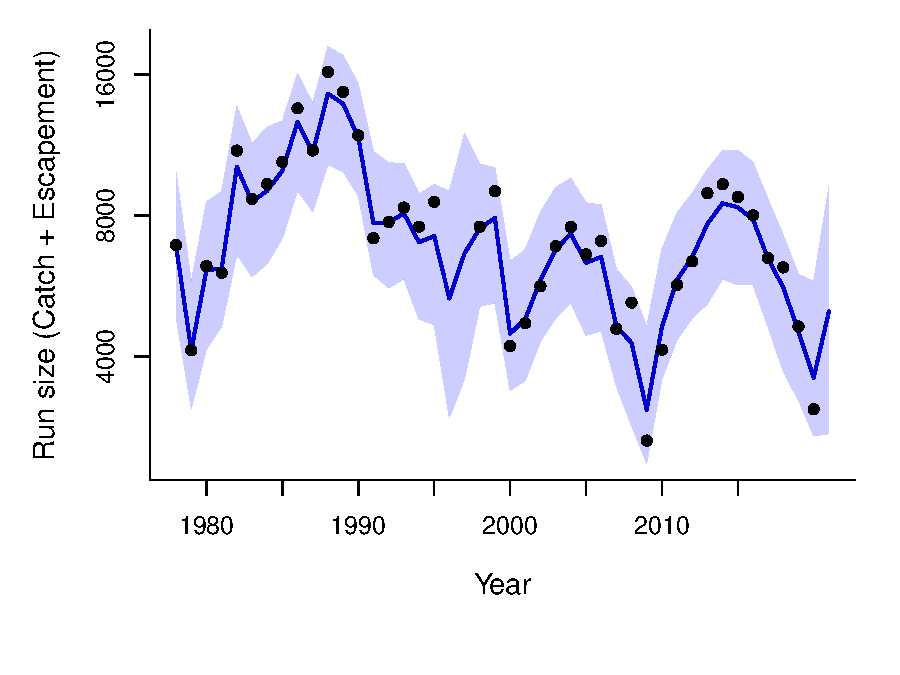
\includegraphics{App_3_Summarize_results_forecast_2020_2021_files/figure-latex/fig_2_run_size-1} \end{center}

Figure 1: Time series of the estimated total population size (catch plus
the adults that escaped to spawn). The observed data are the points; the
solid line is the median estimate and the shaded region indicates the
95\% credible interval.

\hypertarget{terminal-run-size-forecast}{%
\subsection{2021 terminal run size
forecast}\label{terminal-run-size-forecast}}

Here are several percentiles for the 2021 forecast for the total run
size (i.e., catch + escapement).

\begin{Shaded}
\begin{Highlighting}[]
\NormalTok{p_dat <-}\StringTok{ }\NormalTok{mod_res_MA1_AR1[,}\KeywordTok{grep}\NormalTok{(}\StringTok{"Sp"}\NormalTok{, }\KeywordTok{colnames}\NormalTok{(mod_res_MA1_AR1))]}\OperatorTok{*}\NormalTok{model_weights[}\DecValTok{1}\NormalTok{] }\OperatorTok{+}\StringTok{ }\NormalTok{mod_res_AR1[,}\KeywordTok{grep}\NormalTok{(}\StringTok{"Sp"}\NormalTok{, }\KeywordTok{colnames}\NormalTok{(mod_res_AR1))]}\OperatorTok{*}\NormalTok{model_weights[}\DecValTok{2}\NormalTok{]}

\KeywordTok{data.frame}\NormalTok{(}\DataTypeTok{forecast=}\KeywordTok{round}\NormalTok{(}\KeywordTok{quantile}\NormalTok{(p_dat[,n_yrs}\OperatorTok{+}\NormalTok{n_fore],}
                                   \DataTypeTok{probs=}\KeywordTok{c}\NormalTok{(}\FloatTok{0.025}\NormalTok{,}\FloatTok{0.25}\NormalTok{,}\FloatTok{0.5}\NormalTok{,}\FloatTok{0.75}\NormalTok{,}\FloatTok{0.975}\NormalTok{))))}
\end{Highlighting}
\end{Shaded}

\begin{verbatim}
##       forecast
## 2.5%      2735
## 25%       4047
## 50%       4990
## 75%       6183
## 97.5%     9228
\end{verbatim}

\hypertarget{spawner-recruit-relationship}{%
\subsection{Spawner-recruit
relationship}\label{spawner-recruit-relationship}}

Here is the relationship between spawner and subsequent recruits (a),
assuming mean values for all covariates. Gray lines show the median
relationship for each of the 43 years based on \(a_t\). Note that for
plotting purposes only in (b) and (c), the density in the largest bin
for each parameter contains counts for all values greater or equal to
that. Vertical arrows under the x-axes in (b) and (c) indicate the
2.5\textsuperscript{th}, 50\textsuperscript{th}, and
97.5\textsuperscript{th} percentiles.

\begin{Shaded}
\begin{Highlighting}[]
\KeywordTok{layout}\NormalTok{(}\KeywordTok{matrix}\NormalTok{(}\KeywordTok{c}\NormalTok{(}\DecValTok{1}\NormalTok{,}\DecValTok{1}\NormalTok{,}\DecValTok{2}\NormalTok{,}\DecValTok{3}\NormalTok{),}\DecValTok{2}\NormalTok{,}\DecValTok{2}\NormalTok{),}\KeywordTok{c}\NormalTok{(}\DecValTok{3}\NormalTok{,}\DecValTok{2}\NormalTok{),}\KeywordTok{c}\NormalTok{(}\DecValTok{1}\NormalTok{,}\DecValTok{1}\NormalTok{))}
\NormalTok{xoffSet <-}\StringTok{ }\FloatTok{0.05}
\NormalTok{yoffSet <-}\StringTok{ }\FloatTok{0.03}

\CommentTok{## colors for plotting}
\NormalTok{clr <-}\StringTok{ }\KeywordTok{rgb}\NormalTok{(}\DecValTok{100}\NormalTok{, }\DecValTok{0}\NormalTok{, }\DecValTok{200}\NormalTok{,}
           \DataTypeTok{alpha =} \KeywordTok{seq}\NormalTok{(}\DecValTok{200}\NormalTok{, }\DecValTok{100}\NormalTok{,}
                       \DataTypeTok{length.out =}\NormalTok{ age_max}\OperatorTok{-}\NormalTok{age_min}\OperatorTok{+}\NormalTok{n_fore),}
           \DataTypeTok{maxColorValue =} \DecValTok{255}\NormalTok{)}

\CommentTok{## posterior of spawners}
\NormalTok{s_dat <-}\StringTok{ }\NormalTok{mod_res_MA1_AR1[,}\KeywordTok{grep}\NormalTok{(}\StringTok{"Sp"}\NormalTok{, }\KeywordTok{colnames}\NormalTok{(mod_res_MA1_AR1))]}\OperatorTok{*}\NormalTok{model_weights[}\DecValTok{1}\NormalTok{] }\OperatorTok{+}\StringTok{ }\NormalTok{mod_res_AR1[,}\KeywordTok{grep}\NormalTok{(}\StringTok{"Sp"}\NormalTok{, }\KeywordTok{colnames}\NormalTok{(mod_res_AR1))]}\OperatorTok{*}\NormalTok{model_weights[}\DecValTok{2}\NormalTok{]  }

\NormalTok{s_dat <-}\StringTok{ }\KeywordTok{apply}\NormalTok{(s_dat, }\DecValTok{2}\NormalTok{, quantile, CI_vec)}
\NormalTok{s_dat <-}\StringTok{ }\NormalTok{s_dat[, }\DecValTok{1}\OperatorTok{:}\NormalTok{(n_yrs}\OperatorTok{-}\NormalTok{age_min}\OperatorTok{+}\NormalTok{n_fore)]}

\CommentTok{## posterior of recruits}
\NormalTok{r_dat <-}\StringTok{ }\NormalTok{mod_res_MA1_AR1[,}\KeywordTok{grep}\NormalTok{(}\StringTok{"tot_ln_Rec"}\NormalTok{, }\KeywordTok{colnames}\NormalTok{(mod_res_MA1_AR1))]}\OperatorTok{*}\NormalTok{model_weights[}\DecValTok{1}\NormalTok{] }\OperatorTok{+}\StringTok{ }\NormalTok{mod_res_AR1[,}\KeywordTok{grep}\NormalTok{(}\StringTok{"tot_ln_Rec"}\NormalTok{, }\KeywordTok{colnames}\NormalTok{(mod_res_AR1))]}\OperatorTok{*}\NormalTok{model_weights[}\DecValTok{2}\NormalTok{]  }
\NormalTok{r_dat <-}\StringTok{ }\KeywordTok{exp}\NormalTok{(}\KeywordTok{apply}\NormalTok{(r_dat, }\DecValTok{2}\NormalTok{, quantile, CI_vec))}

\CommentTok{## median values for a & b}
\NormalTok{aa <-}\StringTok{ }\NormalTok{mod_res_MA1_AR1[,}\KeywordTok{grep}\NormalTok{(}\StringTok{"ln_BH_a"}\NormalTok{, }\KeywordTok{colnames}\NormalTok{(mod_res_MA1_AR1))]}\OperatorTok{*}\NormalTok{model_weights[}\DecValTok{1}\NormalTok{] }\OperatorTok{+}\StringTok{ }\NormalTok{mod_res_AR1[,}\KeywordTok{grep}\NormalTok{(}\StringTok{"ln_BH_a"}\NormalTok{, }\KeywordTok{colnames}\NormalTok{(mod_res_AR1))]}\OperatorTok{*}\NormalTok{model_weights[}\DecValTok{2}\NormalTok{] }
\NormalTok{aa <-}\StringTok{ }\KeywordTok{apply}\NormalTok{(aa, }\DecValTok{2}\NormalTok{, median)}

\NormalTok{bb <-}\StringTok{ }\NormalTok{mod_res_MA1_AR1[,}\KeywordTok{grep}\NormalTok{(}\StringTok{"beta"}\NormalTok{, }\KeywordTok{colnames}\NormalTok{(mod_res_MA1_AR1))]}\OperatorTok{*}\NormalTok{model_weights[}\DecValTok{1}\NormalTok{] }\OperatorTok{+}\StringTok{ }\NormalTok{mod_res_AR1[,}\KeywordTok{grep}\NormalTok{(}\StringTok{"beta"}\NormalTok{, }\KeywordTok{colnames}\NormalTok{(mod_res_AR1))]}\OperatorTok{*}\NormalTok{model_weights[}\DecValTok{2}\NormalTok{] }
\NormalTok{bb <-}\StringTok{ }\KeywordTok{median}\NormalTok{(bb)}

\CommentTok{## empty plot space for spawner-recruit relationships}
\NormalTok{dd <-}\StringTok{ }\DecValTok{3000}
\NormalTok{yM <-}\StringTok{ }\KeywordTok{around}\NormalTok{(}\KeywordTok{max}\NormalTok{(r_dat), }\StringTok{"ceiling"}\NormalTok{, dd)}
\NormalTok{xM <-}\StringTok{ }\KeywordTok{around}\NormalTok{(}\KeywordTok{max}\NormalTok{(s_dat), }\StringTok{"ceiling"}\NormalTok{, dd)}
\KeywordTok{par}\NormalTok{(}\DataTypeTok{mai =} \KeywordTok{c}\NormalTok{(}\FloatTok{0.8}\NormalTok{,}\FloatTok{0.8}\NormalTok{,}\FloatTok{0.1}\NormalTok{,}\FloatTok{0.1}\NormalTok{), }\DataTypeTok{omi =} \KeywordTok{c}\NormalTok{(}\DecValTok{0}\NormalTok{,}\DecValTok{0}\NormalTok{,}\DecValTok{0}\NormalTok{,}\DecValTok{0}\NormalTok{))}
\KeywordTok{plot}\NormalTok{(s_dat[}\DecValTok{2}\NormalTok{,], r_dat[}\DecValTok{2}\NormalTok{,], }\DataTypeTok{xlim =} \KeywordTok{c}\NormalTok{(}\DecValTok{0}\NormalTok{,xM), }\DataTypeTok{ylim =} \KeywordTok{c}\NormalTok{(}\DecValTok{0}\NormalTok{,yM), }\DataTypeTok{type =} \StringTok{"n"}\NormalTok{,}
     \DataTypeTok{xaxs =} \StringTok{"i"}\NormalTok{, }\DataTypeTok{yaxs =} \StringTok{"i"}\NormalTok{, }\DataTypeTok{cex.lab =} \FloatTok{1.2}\NormalTok{,}
     \DataTypeTok{xlab =} \KeywordTok{expression}\NormalTok{(Spawners}\OperatorTok{~}\NormalTok{(}\DecValTok{10}\OperatorTok{^}\DecValTok{3}\NormalTok{)),}
     \DataTypeTok{ylab =} \KeywordTok{expression}\NormalTok{(Recruits}\OperatorTok{~}\NormalTok{(}\DecValTok{10}\OperatorTok{^}\DecValTok{3}\NormalTok{)),}
     \DataTypeTok{xaxt =} \StringTok{"n"}\NormalTok{, }\DataTypeTok{yaxt =} \StringTok{"n"}\NormalTok{, }\DataTypeTok{bty=}\StringTok{"L"}\NormalTok{)}
\KeywordTok{axis}\NormalTok{(}\DecValTok{1}\NormalTok{, }\DataTypeTok{at =} \KeywordTok{seq}\NormalTok{(}\DecValTok{0}\NormalTok{,xM,dd}\OperatorTok{*}\DecValTok{2}\NormalTok{), }\DataTypeTok{labels =} \KeywordTok{seq}\NormalTok{(}\DecValTok{0}\NormalTok{,xM,dd}\OperatorTok{*}\DecValTok{2}\NormalTok{)}\OperatorTok{/}\DecValTok{1000}\NormalTok{)}
\KeywordTok{axis}\NormalTok{(}\DecValTok{2}\NormalTok{, }\DataTypeTok{at =} \KeywordTok{seq}\NormalTok{(}\DecValTok{0}\NormalTok{,yM,dd}\OperatorTok{*}\DecValTok{2}\NormalTok{), }\DataTypeTok{labels =} \KeywordTok{seq}\NormalTok{(}\DecValTok{0}\NormalTok{,yM,dd}\OperatorTok{*}\DecValTok{2}\NormalTok{)}\OperatorTok{/}\DecValTok{1000}\NormalTok{, }\DataTypeTok{las=}\DecValTok{1}\NormalTok{)}
\ControlFlowTok{for}\NormalTok{(i }\ControlFlowTok{in} \DecValTok{1}\OperatorTok{:}\KeywordTok{length}\NormalTok{(aa)) \{}
  \KeywordTok{lines}\NormalTok{(}\KeywordTok{exp}\NormalTok{(aa[i]) }\OperatorTok{*}\StringTok{ }\KeywordTok{seq}\NormalTok{(}\DecValTok{0}\NormalTok{,xM) }\OperatorTok{/}\StringTok{ }\NormalTok{(}\DecValTok{1} \OperatorTok{+}\StringTok{ }\NormalTok{bb }\OperatorTok{*}\StringTok{ }\KeywordTok{seq}\NormalTok{(}\DecValTok{0}\NormalTok{,xM)),}
        \DataTypeTok{col =} \StringTok{"darkgray"}\NormalTok{)}
\NormalTok{\}}
\KeywordTok{abline}\NormalTok{(}\DataTypeTok{a =} \DecValTok{0}\NormalTok{,}\DataTypeTok{b =} \DecValTok{1}\NormalTok{,}\DataTypeTok{lty =} \StringTok{"dashed"}\NormalTok{)}

\CommentTok{## add S-R estimates and medians}
\NormalTok{nCB <-}\StringTok{ }\NormalTok{n_yrs}\OperatorTok{-}\NormalTok{age_max}
\CommentTok{## years with complete returns}
\KeywordTok{points}\NormalTok{(s_dat[}\DecValTok{2}\NormalTok{, }\DecValTok{1}\OperatorTok{:}\NormalTok{nCB], r_dat[}\DecValTok{2}\NormalTok{, }\DecValTok{1}\OperatorTok{:}\NormalTok{nCB],}
       \DataTypeTok{xlim =} \KeywordTok{c}\NormalTok{(}\DecValTok{0}\NormalTok{,xM), }\DataTypeTok{ylim =} \KeywordTok{c}\NormalTok{(}\DecValTok{0}\NormalTok{,yM),}
       \DataTypeTok{pch =} \DecValTok{16}\NormalTok{, }\DataTypeTok{col =} \StringTok{"blue3"}\NormalTok{)}
\KeywordTok{segments}\NormalTok{(s_dat[}\DecValTok{2}\NormalTok{, }\DecValTok{1}\OperatorTok{:}\NormalTok{nCB], r_dat[}\DecValTok{1}\NormalTok{, }\DecValTok{1}\OperatorTok{:}\NormalTok{nCB],}
\NormalTok{         s_dat[}\DecValTok{2}\NormalTok{, }\DecValTok{1}\OperatorTok{:}\NormalTok{nCB], r_dat[}\DecValTok{3}\NormalTok{, }\DecValTok{1}\OperatorTok{:}\NormalTok{nCB],}
         \DataTypeTok{col =} \StringTok{"blue3"}\NormalTok{)}
\KeywordTok{segments}\NormalTok{(s_dat[}\DecValTok{1}\NormalTok{, }\DecValTok{1}\OperatorTok{:}\NormalTok{nCB], r_dat[}\DecValTok{2}\NormalTok{, }\DecValTok{1}\OperatorTok{:}\NormalTok{nCB],}
\NormalTok{         s_dat[}\DecValTok{3}\NormalTok{, }\DecValTok{1}\OperatorTok{:}\NormalTok{nCB], r_dat[}\DecValTok{2}\NormalTok{, }\DecValTok{1}\OperatorTok{:}\NormalTok{nCB],}
         \DataTypeTok{col =} \StringTok{"blue3"}\NormalTok{)}
\NormalTok{nTB <-}\StringTok{ }\KeywordTok{dim}\NormalTok{(s_dat)[}\DecValTok{2}\NormalTok{]}
\CommentTok{## years with incomplete returns}
\KeywordTok{segments}\NormalTok{(s_dat[}\DecValTok{2}\NormalTok{, (nCB}\OperatorTok{+}\DecValTok{1}\NormalTok{)}\OperatorTok{:}\NormalTok{nTB], r_dat[}\DecValTok{1}\NormalTok{, (nCB}\OperatorTok{+}\DecValTok{1}\NormalTok{)}\OperatorTok{:}\NormalTok{nTB],}
\NormalTok{         s_dat[}\DecValTok{2}\NormalTok{, (nCB}\OperatorTok{+}\DecValTok{1}\NormalTok{)}\OperatorTok{:}\NormalTok{nTB], r_dat[}\DecValTok{3}\NormalTok{, (nCB}\OperatorTok{+}\DecValTok{1}\NormalTok{)}\OperatorTok{:}\NormalTok{nTB],}
         \DataTypeTok{col =}\NormalTok{ clr)}
\KeywordTok{segments}\NormalTok{(s_dat[}\DecValTok{1}\NormalTok{, (nCB}\OperatorTok{+}\DecValTok{1}\NormalTok{)}\OperatorTok{:}\NormalTok{nTB], r_dat[}\DecValTok{2}\NormalTok{, (nCB}\OperatorTok{+}\DecValTok{1}\NormalTok{)}\OperatorTok{:}\NormalTok{nTB],}
\NormalTok{         s_dat[}\DecValTok{3}\NormalTok{, (nCB}\OperatorTok{+}\DecValTok{1}\NormalTok{)}\OperatorTok{:}\NormalTok{nTB], r_dat[}\DecValTok{2}\NormalTok{, (nCB}\OperatorTok{+}\DecValTok{1}\NormalTok{)}\OperatorTok{:}\NormalTok{nTB],}
         \DataTypeTok{col =}\NormalTok{ clr)}
\KeywordTok{points}\NormalTok{(s_dat[}\DecValTok{2}\NormalTok{, (nCB}\OperatorTok{+}\DecValTok{1}\NormalTok{)}\OperatorTok{:}\NormalTok{nTB],r_dat[}\DecValTok{2}\NormalTok{, (nCB}\OperatorTok{+}\DecValTok{1}\NormalTok{)}\OperatorTok{:}\NormalTok{nTB],}
       \DataTypeTok{xlim =} \KeywordTok{c}\NormalTok{(}\DecValTok{0}\NormalTok{,xM), }\DataTypeTok{ylim =} \KeywordTok{c}\NormalTok{(}\DecValTok{0}\NormalTok{,yM),}
       \DataTypeTok{pch =} \DecValTok{16}\NormalTok{, }\DataTypeTok{col =}\NormalTok{ clr)}
\KeywordTok{text}\NormalTok{(}\DataTypeTok{x =} \KeywordTok{par}\NormalTok{()}\OperatorTok{$}\NormalTok{usr[}\DecValTok{1}\NormalTok{] }\OperatorTok{+}\StringTok{ }\KeywordTok{diff}\NormalTok{(}\KeywordTok{par}\NormalTok{()}\OperatorTok{$}\NormalTok{usr[}\DecValTok{1}\OperatorTok{:}\DecValTok{2}\NormalTok{]) }\OperatorTok{*}\StringTok{ }\NormalTok{xoffSet,}
     \DataTypeTok{y =} \KeywordTok{par}\NormalTok{()}\OperatorTok{$}\NormalTok{usr[}\DecValTok{4}\NormalTok{] }\OperatorTok{-}\StringTok{ }\KeywordTok{diff}\NormalTok{(}\KeywordTok{par}\NormalTok{()}\OperatorTok{$}\NormalTok{usr[}\DecValTok{3}\OperatorTok{:}\DecValTok{4}\NormalTok{]) }\OperatorTok{*}\StringTok{ }\NormalTok{yoffSet,}
     \StringTok{"(a)"}\NormalTok{)}

\CommentTok{## posterior for alpha}
\NormalTok{clr <-}\StringTok{ }\KeywordTok{rgb}\NormalTok{(}\DecValTok{0}\NormalTok{, }\DecValTok{0}\NormalTok{, }\DecValTok{255}\NormalTok{, }\DataTypeTok{alpha =} \DecValTok{50}\NormalTok{, }\DataTypeTok{maxColorValue =} \DecValTok{255}\NormalTok{)}
\NormalTok{a_thresh <-}\StringTok{ }\DecValTok{59}
\KeywordTok{par}\NormalTok{(}\DataTypeTok{mai =} \KeywordTok{c}\NormalTok{(}\FloatTok{0.8}\NormalTok{,}\FloatTok{0.4}\NormalTok{,}\FloatTok{0.3}\NormalTok{,}\FloatTok{0.1}\NormalTok{))}
\CommentTok{## B-H alpha}
\NormalTok{R_alpha_est <-}\StringTok{ }\NormalTok{mod_res_MA1_AR1[,}\KeywordTok{grep}\NormalTok{(}\StringTok{"alpha"}\NormalTok{, }\KeywordTok{colnames}\NormalTok{(mod_res_MA1_AR1))]}\OperatorTok{*}\NormalTok{model_weights[}\DecValTok{1}\NormalTok{] }\OperatorTok{+}\StringTok{ }\NormalTok{mod_res_AR1[,}\KeywordTok{grep}\NormalTok{(}\StringTok{"alpha"}\NormalTok{, }\KeywordTok{colnames}\NormalTok{(mod_res_AR1))]}\OperatorTok{*}\NormalTok{model_weights[}\DecValTok{2}\NormalTok{] }
\NormalTok{alphaCI <-}\StringTok{ }\KeywordTok{quantile}\NormalTok{(R_alpha_est, CI_vec)}
\NormalTok{R_alpha_est[R_alpha_est }\OperatorTok{>}\StringTok{ }\NormalTok{a_thresh] <-}\StringTok{ }\NormalTok{a_thresh}
\KeywordTok{hist}\NormalTok{(R_alpha_est, }\DataTypeTok{freq =} \OtherTok{FALSE}\NormalTok{, }\DataTypeTok{breaks =} \KeywordTok{seq}\NormalTok{(}\DecValTok{0}\NormalTok{, a_thresh}\OperatorTok{+}\DecValTok{1}\NormalTok{, }\DecValTok{2}\NormalTok{),}
     \DataTypeTok{col =}\NormalTok{ clr, }\DataTypeTok{border =} \StringTok{"blue3"}\NormalTok{,}
     \DataTypeTok{xlab =} \StringTok{""}\NormalTok{, }\DataTypeTok{ylab =} \StringTok{""}\NormalTok{, }\DataTypeTok{main =} \StringTok{""}\NormalTok{, }\DataTypeTok{cex.lab =} \FloatTok{1.2}\NormalTok{, }\DataTypeTok{yaxt =} \StringTok{"n"}\NormalTok{)}
\NormalTok{aHt <-}\StringTok{ }\NormalTok{(}\KeywordTok{par}\NormalTok{()}\OperatorTok{$}\NormalTok{usr[}\DecValTok{4}\NormalTok{]}\OperatorTok{-}\KeywordTok{par}\NormalTok{()}\OperatorTok{$}\NormalTok{usr[}\DecValTok{3}\NormalTok{])}\OperatorTok{/}\DecValTok{12}
\KeywordTok{arrows}\NormalTok{(alphaCI, }\KeywordTok{par}\NormalTok{()}\OperatorTok{$}\NormalTok{usr[}\DecValTok{3}\NormalTok{], alphaCI,}\KeywordTok{par}\NormalTok{()}\OperatorTok{$}\NormalTok{usr[}\DecValTok{3}\NormalTok{]}\OperatorTok{-}\NormalTok{aHt,}
       \DataTypeTok{code =} \DecValTok{1}\NormalTok{, }\DataTypeTok{length =} \FloatTok{0.05}\NormalTok{, }\DataTypeTok{xpd =} \OtherTok{NA}\NormalTok{, }\DataTypeTok{col =} \StringTok{"blue3"}\NormalTok{, }\DataTypeTok{lwd =} \FloatTok{1.5}\NormalTok{)}
\KeywordTok{mtext}\NormalTok{(}\KeywordTok{expression}\NormalTok{(Instrinsic}\OperatorTok{~}\NormalTok{productivity}\OperatorTok{~}\NormalTok{(alpha)), }\DecValTok{1}\NormalTok{, }\DataTypeTok{line =} \DecValTok{3}\NormalTok{, }\DataTypeTok{cex =} \DecValTok{1}\NormalTok{)}
\KeywordTok{text}\NormalTok{(}\DataTypeTok{x =} \KeywordTok{par}\NormalTok{()}\OperatorTok{$}\NormalTok{usr[}\DecValTok{1}\NormalTok{],}
     \DataTypeTok{y =} \KeywordTok{par}\NormalTok{()}\OperatorTok{$}\NormalTok{usr[}\DecValTok{4}\NormalTok{] }\OperatorTok{*}\StringTok{ }\FloatTok{1.05}\NormalTok{,}
     \StringTok{"(b)"}\NormalTok{, }\DataTypeTok{xpd=}\OtherTok{NA}\NormalTok{)}

\CommentTok{## posterior for K}
\KeywordTok{par}\NormalTok{(}\DataTypeTok{mai =} \KeywordTok{c}\NormalTok{(}\FloatTok{0.8}\NormalTok{,}\FloatTok{0.4}\NormalTok{,}\FloatTok{0.3}\NormalTok{,}\FloatTok{0.1}\NormalTok{))}
\NormalTok{aa <-}\StringTok{ }\NormalTok{mod_res_MA1_AR1[,}\KeywordTok{grep}\NormalTok{(}\StringTok{"alpha"}\NormalTok{, }\KeywordTok{colnames}\NormalTok{(mod_res_MA1_AR1))]}\OperatorTok{*}\NormalTok{model_weights[}\DecValTok{1}\NormalTok{] }\OperatorTok{+}\StringTok{ }\NormalTok{mod_res_AR1[,}\KeywordTok{grep}\NormalTok{(}\StringTok{"alpha"}\NormalTok{, }\KeywordTok{colnames}\NormalTok{(mod_res_AR1))]}\OperatorTok{*}\NormalTok{model_weights[}\DecValTok{2}\NormalTok{] }
\NormalTok{bb <-}\StringTok{ }\NormalTok{mod_res_MA1_AR1[,}\KeywordTok{grep}\NormalTok{(}\StringTok{"beta"}\NormalTok{, }\KeywordTok{colnames}\NormalTok{(mod_res_MA1_AR1))]}\OperatorTok{*}\NormalTok{model_weights[}\DecValTok{1}\NormalTok{] }\OperatorTok{+}\StringTok{ }\NormalTok{mod_res_AR1[,}\KeywordTok{grep}\NormalTok{(}\StringTok{"beta"}\NormalTok{, }\KeywordTok{colnames}\NormalTok{(mod_res_AR1))]}\OperatorTok{*}\NormalTok{model_weights[}\DecValTok{2}\NormalTok{] }
\CommentTok{## K in 1000s}
\NormalTok{R_b_est <-}\StringTok{ }\NormalTok{(aa}\DecValTok{-1}\NormalTok{) }\OperatorTok{/}\StringTok{ }\NormalTok{bb }\OperatorTok{/}\StringTok{ }\DecValTok{1000}
\NormalTok{R_b_est <-}\StringTok{ }\NormalTok{R_b_est[R_b_est }\OperatorTok{>}\StringTok{ }\DecValTok{0}\NormalTok{]}
\NormalTok{R_b_CI <-}\StringTok{ }\KeywordTok{quantile}\NormalTok{(R_b_est, CI_vec)}
\CommentTok{## pile into last ban for plotting}
\NormalTok{R_b_est[R_b_est }\OperatorTok{>}\StringTok{ }\DecValTok{13}\NormalTok{] <-}\StringTok{ }\DecValTok{13}
\NormalTok{brks <-}\StringTok{ }\KeywordTok{seq}\NormalTok{(}\KeywordTok{around}\NormalTok{(}\KeywordTok{min}\NormalTok{(R_b_est), }\StringTok{"floor"}\NormalTok{),}
            \KeywordTok{around}\NormalTok{(}\KeywordTok{max}\NormalTok{(R_b_est), }\StringTok{"ceiling"}\NormalTok{),}
            \DataTypeTok{length.out =} \KeywordTok{length}\NormalTok{(}\KeywordTok{seq}\NormalTok{(}\DecValTok{0}\NormalTok{, a_thresh, }\DecValTok{2}\NormalTok{)))}
\KeywordTok{hist}\NormalTok{(R_b_est, }\DataTypeTok{freq =} \OtherTok{FALSE}\NormalTok{, }\DataTypeTok{breaks =}\NormalTok{ brks, }\DataTypeTok{col =}\NormalTok{ clr, }\DataTypeTok{border =} \StringTok{"blue3"}\NormalTok{,}
     \DataTypeTok{xlab =} \StringTok{""}\NormalTok{, }\DataTypeTok{xaxt =} \StringTok{"n"}\NormalTok{, }\DataTypeTok{yaxt =} \StringTok{"n"}\NormalTok{,}
     \DataTypeTok{main =} \StringTok{""}\NormalTok{, }\DataTypeTok{ylab =} \StringTok{""}\NormalTok{, }\DataTypeTok{cex.lab =} \FloatTok{1.2}\NormalTok{)}
\KeywordTok{axis}\NormalTok{(}\DecValTok{1}\NormalTok{, }\DataTypeTok{at =} \KeywordTok{seq}\NormalTok{(}\KeywordTok{around}\NormalTok{(}\KeywordTok{min}\NormalTok{(R_b_est), }\StringTok{"floor"}\NormalTok{),}
                 \KeywordTok{around}\NormalTok{(}\KeywordTok{max}\NormalTok{(R_b_est), }\StringTok{"ceiling"}\NormalTok{),}
                 \DecValTok{2}\NormalTok{))}
\NormalTok{aHt <-}\StringTok{ }\NormalTok{(}\KeywordTok{par}\NormalTok{()}\OperatorTok{$}\NormalTok{usr[}\DecValTok{4}\NormalTok{] }\OperatorTok{-}\StringTok{ }\KeywordTok{par}\NormalTok{()}\OperatorTok{$}\NormalTok{usr[}\DecValTok{3}\NormalTok{]) }\OperatorTok{/}\StringTok{ }\DecValTok{12}
\KeywordTok{arrows}\NormalTok{(R_b_CI, }\KeywordTok{par}\NormalTok{()}\OperatorTok{$}\NormalTok{usr[}\DecValTok{3}\NormalTok{], R_b_CI,}\KeywordTok{par}\NormalTok{()}\OperatorTok{$}\NormalTok{usr[}\DecValTok{3}\NormalTok{]}\OperatorTok{-}\NormalTok{aHt,}
       \DataTypeTok{code =} \DecValTok{1}\NormalTok{, }\DataTypeTok{length =} \FloatTok{0.05}\NormalTok{, }\DataTypeTok{xpd =} \OtherTok{NA}\NormalTok{, }\DataTypeTok{col =} \StringTok{"blue3"}\NormalTok{, }\DataTypeTok{lwd =} \FloatTok{1.5}\NormalTok{)}
\KeywordTok{mtext}\NormalTok{(}\KeywordTok{expression}\NormalTok{(}\KeywordTok{paste}\NormalTok{(}\StringTok{"Carrying capacity ("}\NormalTok{,}\KeywordTok{italic}\NormalTok{(K),}\StringTok{", "}\NormalTok{,}\DecValTok{10}\OperatorTok{^}\DecValTok{3}\NormalTok{,}\StringTok{")"}\NormalTok{)),}
      \DataTypeTok{side =} \DecValTok{1}\NormalTok{, }\DataTypeTok{line =} \DecValTok{3}\NormalTok{, }\DataTypeTok{cex =} \DecValTok{1}\NormalTok{)}
\KeywordTok{text}\NormalTok{(}\DataTypeTok{x =} \KeywordTok{par}\NormalTok{()}\OperatorTok{$}\NormalTok{usr[}\DecValTok{1}\NormalTok{], }
     \DataTypeTok{y =} \KeywordTok{par}\NormalTok{()}\OperatorTok{$}\NormalTok{usr[}\DecValTok{4}\NormalTok{] }\OperatorTok{*}\StringTok{ }\FloatTok{1.05}\NormalTok{,}
     \StringTok{"(c)"}\NormalTok{, }\DataTypeTok{xpd=}\OtherTok{NA}\NormalTok{)}
\end{Highlighting}
\end{Shaded}

\begin{center}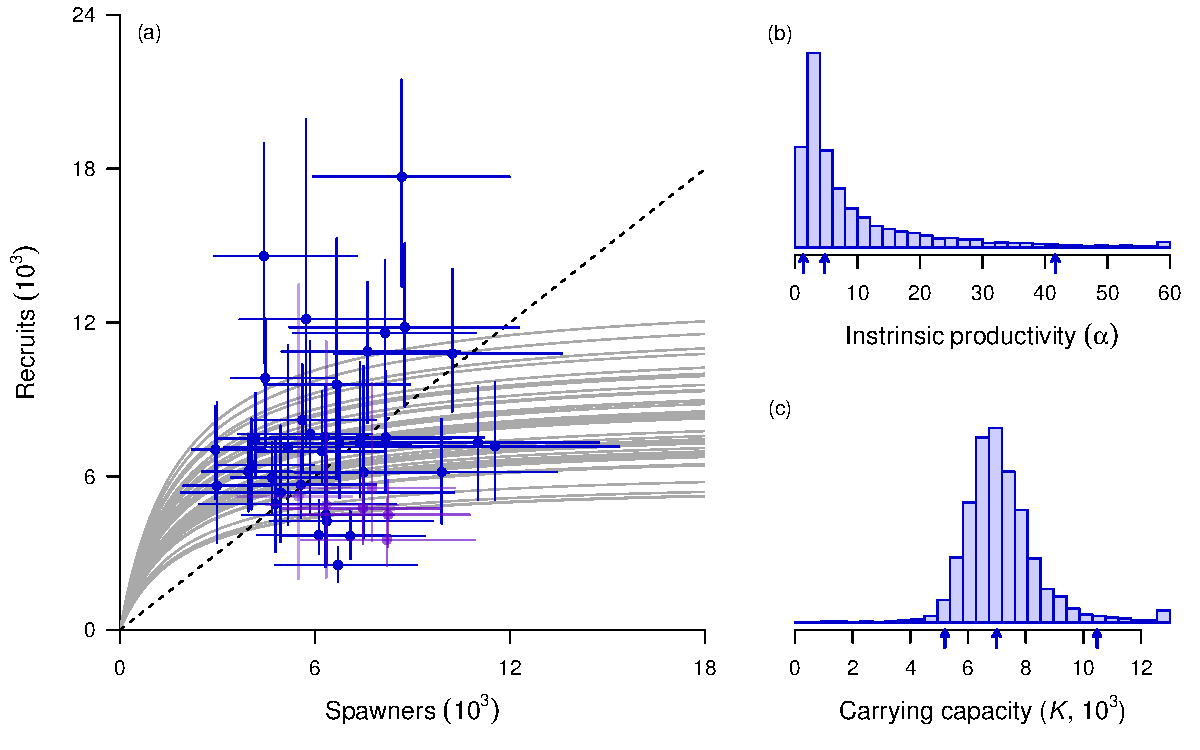
\includegraphics{App_3_Summarize_results_forecast_2020_2021_files/figure-latex/fig_3_S-R-1} \end{center}

Figure 2: Relationship between the number of spawning adults and their
subsequent surviving offspring (recruits), assuming mean values for all
covariates (a); and the estimated posterior distributions for the
intrinsic productivity (b) and carrying capacity (c). Points in (a) are
medians of the posterior estimates; error bars indicate the 95\%
credible intervals. Blue points are for estimates with complete broods;
purple points are for the most recent years with incomplete broods. Gray
lines show the median relationship for each of the 41 years in the time
series based on annual model estimates of productivity. Note that for
plotting purposes only in (b) and (c), the density in the largest bin
for each parameter contains counts for all values greater than or equal
to it. Vertical arrows under the x-axes in (b) and (c) indicate the
2.5\(^\text{th}\), 50\(^\text{th}\), and 97.5\(^\text{th}\) percentiles.

Here are summaries of the posterior distributions for \(\alpha\) and
\(K\).

\begin{Shaded}
\begin{Highlighting}[]
\CommentTok{## intrinsic productivity}
\KeywordTok{round}\NormalTok{(alphaCI, }\DecValTok{2}\NormalTok{)}
\end{Highlighting}
\end{Shaded}

\begin{verbatim}
##  2.5%   50% 97.5% 
##  1.34  4.76 41.66
\end{verbatim}

\begin{Shaded}
\begin{Highlighting}[]
\CommentTok{## carrying capacity}
\KeywordTok{round}\NormalTok{(R_b_CI, }\DecValTok{2}\NormalTok{)}
\end{Highlighting}
\end{Shaded}

\begin{verbatim}
##  2.5%   50% 97.5% 
##  5.20  6.99 10.47
\end{verbatim}

\hypertarget{covariate-effects}{%
\subsection{Covariate effects}\label{covariate-effects}}

Here are time series plots of the covariates (a-c) and histograms of
their effects on productivity (d-f).

\begin{Shaded}
\begin{Highlighting}[]
\NormalTok{clr <-}\StringTok{ }\KeywordTok{rgb}\NormalTok{(}\DecValTok{0}\NormalTok{, }\DecValTok{0}\NormalTok{, }\DecValTok{255}\NormalTok{, }\DataTypeTok{alpha =} \DecValTok{50}\NormalTok{, }\DataTypeTok{maxColorValue =} \DecValTok{255}\NormalTok{)}
\NormalTok{xoffSet <-}\StringTok{ }\FloatTok{0.04}
\NormalTok{yoffSet <-}\StringTok{ }\FloatTok{0.03}

\KeywordTok{par}\NormalTok{(}\DataTypeTok{mfrow=}\KeywordTok{c}\NormalTok{(n_cov,}\DecValTok{2}\NormalTok{), }\DataTypeTok{mai=}\KeywordTok{c}\NormalTok{(}\FloatTok{0.4}\NormalTok{,}\FloatTok{0.2}\NormalTok{,}\FloatTok{0.1}\NormalTok{,}\FloatTok{0.1}\NormalTok{), }\DataTypeTok{omi=}\KeywordTok{c}\NormalTok{(}\FloatTok{0.2}\NormalTok{,}\FloatTok{0.5}\NormalTok{,}\DecValTok{0}\NormalTok{,}\DecValTok{0}\NormalTok{))}

\NormalTok{c_est <-}\StringTok{ }\NormalTok{mod_res_MA1_AR1[,}\KeywordTok{grep}\NormalTok{(}\StringTok{"gamma"}\NormalTok{, }\KeywordTok{colnames}\NormalTok{(mod_res_MA1_AR1))]}\OperatorTok{*}\NormalTok{model_weights[}\DecValTok{1}\NormalTok{] }\OperatorTok{+}\StringTok{ }\NormalTok{mod_res_AR1[,}\KeywordTok{grep}\NormalTok{(}\StringTok{"gamma"}\NormalTok{, }\KeywordTok{colnames}\NormalTok{(mod_res_AR1))]}\OperatorTok{*}\NormalTok{model_weights[}\DecValTok{2}\NormalTok{] }

\NormalTok{ylN <-}\StringTok{ }\KeywordTok{floor}\NormalTok{(}\KeywordTok{min}\NormalTok{(c_est)}\OperatorTok{*}\DecValTok{10}\NormalTok{)}\OperatorTok{/}\DecValTok{10}
\NormalTok{ylM <-}\StringTok{ }\KeywordTok{ceiling}\NormalTok{(}\KeywordTok{max}\NormalTok{(c_est)}\OperatorTok{*}\DecValTok{10}\NormalTok{)}\OperatorTok{/}\DecValTok{10}
\NormalTok{brks <-}\StringTok{ }\KeywordTok{seq}\NormalTok{(ylN,ylM,}\DataTypeTok{length.out=}\KeywordTok{diff}\NormalTok{(}\KeywordTok{c}\NormalTok{(ylN,ylM))}\OperatorTok{*}\DecValTok{40}\OperatorTok{+}\DecValTok{1}\NormalTok{)}
\NormalTok{t_idx <-}\StringTok{ }\KeywordTok{seq}\NormalTok{(yr_frst,}\DataTypeTok{length.out=}\NormalTok{n_yrs}\OperatorTok{-}\NormalTok{age_min}\OperatorTok{+}\NormalTok{n_fore)}
\NormalTok{dat_cvrs <-}\StringTok{ }\KeywordTok{as.matrix}\NormalTok{(dat_cvrs[}\KeywordTok{seq}\NormalTok{(}\KeywordTok{length}\NormalTok{(t_idx)),])}

\ControlFlowTok{for}\NormalTok{(i }\ControlFlowTok{in} \DecValTok{1}\OperatorTok{:}\NormalTok{n_cov) \{}
  \ControlFlowTok{if}\NormalTok{(i}\OperatorTok{==}\DecValTok{4}\NormalTok{) \{}
\NormalTok{    dat_cvrs[,i}\OperatorTok{+}\DecValTok{1}\NormalTok{] <-}\StringTok{ }\NormalTok{dat_cvrs[,i}\OperatorTok{+}\DecValTok{1}\NormalTok{]}\OperatorTok{/}\DecValTok{1000}
\NormalTok{  \}}
  \CommentTok{## plot covar ts}
  \KeywordTok{plot}\NormalTok{(dat_cvrs[, }\StringTok{"year"}\NormalTok{], dat_cvrs[, i}\OperatorTok{+}\DecValTok{1}\NormalTok{],}
       \DataTypeTok{pch =} \DecValTok{16}\NormalTok{, }\DataTypeTok{col =} \StringTok{"blue3"}\NormalTok{, }\DataTypeTok{type =} \StringTok{"o"}\NormalTok{,}
       \DataTypeTok{xlab =} \StringTok{""}\NormalTok{, }\DataTypeTok{ylab =} \StringTok{""}\NormalTok{, }\DataTypeTok{main =} \StringTok{""}\NormalTok{, }\DataTypeTok{bty =} \StringTok{"L"}\NormalTok{,}
       \DataTypeTok{cex.axis =} \FloatTok{1.2}\NormalTok{)}
  \KeywordTok{text}\NormalTok{(}\DataTypeTok{x =} \KeywordTok{par}\NormalTok{()}\OperatorTok{$}\NormalTok{usr[}\DecValTok{1}\NormalTok{] }\OperatorTok{+}\StringTok{ }\KeywordTok{diff}\NormalTok{(}\KeywordTok{par}\NormalTok{()}\OperatorTok{$}\NormalTok{usr[}\DecValTok{1}\OperatorTok{:}\DecValTok{2}\NormalTok{]) }\OperatorTok{*}\StringTok{ }\NormalTok{xoffSet,}
       \DataTypeTok{y =} \KeywordTok{par}\NormalTok{()}\OperatorTok{$}\NormalTok{usr[}\DecValTok{4}\NormalTok{] }\OperatorTok{-}\StringTok{ }\KeywordTok{diff}\NormalTok{(}\KeywordTok{par}\NormalTok{()}\OperatorTok{$}\NormalTok{usr[}\DecValTok{3}\OperatorTok{:}\DecValTok{4}\NormalTok{]) }\OperatorTok{*}\StringTok{ }\NormalTok{yoffSet,}
       \KeywordTok{paste0}\NormalTok{(}\StringTok{"("}\NormalTok{,letters[i],}\StringTok{")"}\NormalTok{),}
       \DataTypeTok{cex =} \FloatTok{1.2}\NormalTok{)}
  \KeywordTok{mtext}\NormalTok{(}\DataTypeTok{side =} \DecValTok{2}\NormalTok{, cov_names[i], }\DataTypeTok{line =} \DecValTok{3}\NormalTok{, }\DataTypeTok{cex =} \FloatTok{1.2}\NormalTok{)}
  \ControlFlowTok{if}\NormalTok{(i }\OperatorTok{==}\StringTok{ }\NormalTok{n_cov) \{}
    \KeywordTok{mtext}\NormalTok{(}\DataTypeTok{side =} \DecValTok{1}\NormalTok{, }\StringTok{"Brood year"}\NormalTok{, }\DataTypeTok{line =} \DecValTok{3}\NormalTok{)}
\NormalTok{  \}}
  \CommentTok{## plot covar effect}
  \KeywordTok{hist}\NormalTok{(c_est[,i],}
       \DataTypeTok{freq =} \OtherTok{FALSE}\NormalTok{, }\DataTypeTok{breaks =}\NormalTok{ brks, }\DataTypeTok{col =}\NormalTok{ clr, }\DataTypeTok{border =}\StringTok{" blue3"}\NormalTok{,}
       \DataTypeTok{xlab =} \StringTok{""}\NormalTok{, }\DataTypeTok{yaxt =} \StringTok{"n"}\NormalTok{, }\DataTypeTok{main =} \StringTok{""}\NormalTok{, }\DataTypeTok{ylab =} \StringTok{""}\NormalTok{, }\DataTypeTok{cex.axis =} \FloatTok{1.2}\NormalTok{)}
\NormalTok{  c_CI <-}\StringTok{ }\KeywordTok{quantile}\NormalTok{(c_est[,i],CI_vec)}
\NormalTok{  aHt <-}\StringTok{ }\NormalTok{(}\KeywordTok{par}\NormalTok{()}\OperatorTok{$}\NormalTok{usr[}\DecValTok{4}\NormalTok{]}\OperatorTok{-}\KeywordTok{par}\NormalTok{()}\OperatorTok{$}\NormalTok{usr[}\DecValTok{3}\NormalTok{])}\OperatorTok{/}\DecValTok{20}
  \KeywordTok{arrows}\NormalTok{(c_CI, }\KeywordTok{par}\NormalTok{()}\OperatorTok{$}\NormalTok{usr[}\DecValTok{3}\NormalTok{]}\OperatorTok{-}\FloatTok{0.005}\NormalTok{, c_CI, }\KeywordTok{par}\NormalTok{()}\OperatorTok{$}\NormalTok{usr[}\DecValTok{3}\NormalTok{] }\OperatorTok{-}\StringTok{ }\NormalTok{aHt,}
         \DataTypeTok{code =} \DecValTok{1}\NormalTok{,}\DataTypeTok{length =} \FloatTok{0.05}\NormalTok{, }\DataTypeTok{xpd =} \OtherTok{NA}\NormalTok{, }\DataTypeTok{col =} \StringTok{"blue3"}\NormalTok{, }\DataTypeTok{lwd =} \FloatTok{1.5}\NormalTok{)}
  \KeywordTok{abline}\NormalTok{(}\DataTypeTok{v =} \DecValTok{0}\NormalTok{, }\DataTypeTok{lty =} \StringTok{"dashed"}\NormalTok{)}
  \KeywordTok{text}\NormalTok{(}\DataTypeTok{x =} \KeywordTok{par}\NormalTok{()}\OperatorTok{$}\NormalTok{usr[}\DecValTok{1}\NormalTok{] }\OperatorTok{+}\StringTok{ }\KeywordTok{diff}\NormalTok{(}\KeywordTok{par}\NormalTok{()}\OperatorTok{$}\NormalTok{usr[}\DecValTok{1}\OperatorTok{:}\DecValTok{2}\NormalTok{]) }\OperatorTok{*}\StringTok{ }\NormalTok{xoffSet,}
       \DataTypeTok{y =} \KeywordTok{par}\NormalTok{()}\OperatorTok{$}\NormalTok{usr[}\DecValTok{4}\NormalTok{] }\OperatorTok{-}\StringTok{ }\KeywordTok{diff}\NormalTok{(}\KeywordTok{par}\NormalTok{()}\OperatorTok{$}\NormalTok{usr[}\DecValTok{3}\OperatorTok{:}\DecValTok{4}\NormalTok{]) }\OperatorTok{*}\StringTok{ }\NormalTok{yoffSet,}
       \KeywordTok{paste0}\NormalTok{(}\StringTok{"("}\NormalTok{,letters[i}\OperatorTok{+}\NormalTok{n_cov],}\StringTok{")"}\NormalTok{),}
       \DataTypeTok{cex =} \FloatTok{1.2}\NormalTok{)}
  \ControlFlowTok{if}\NormalTok{(i }\OperatorTok{==}\StringTok{ }\NormalTok{n_cov) \{ }\KeywordTok{mtext}\NormalTok{(}\DataTypeTok{side =} \DecValTok{1}\NormalTok{,}\StringTok{"Effect size"}\NormalTok{, }\DataTypeTok{line =} \DecValTok{3}\NormalTok{) \}}
\NormalTok{\}}
\end{Highlighting}
\end{Shaded}

\begin{center}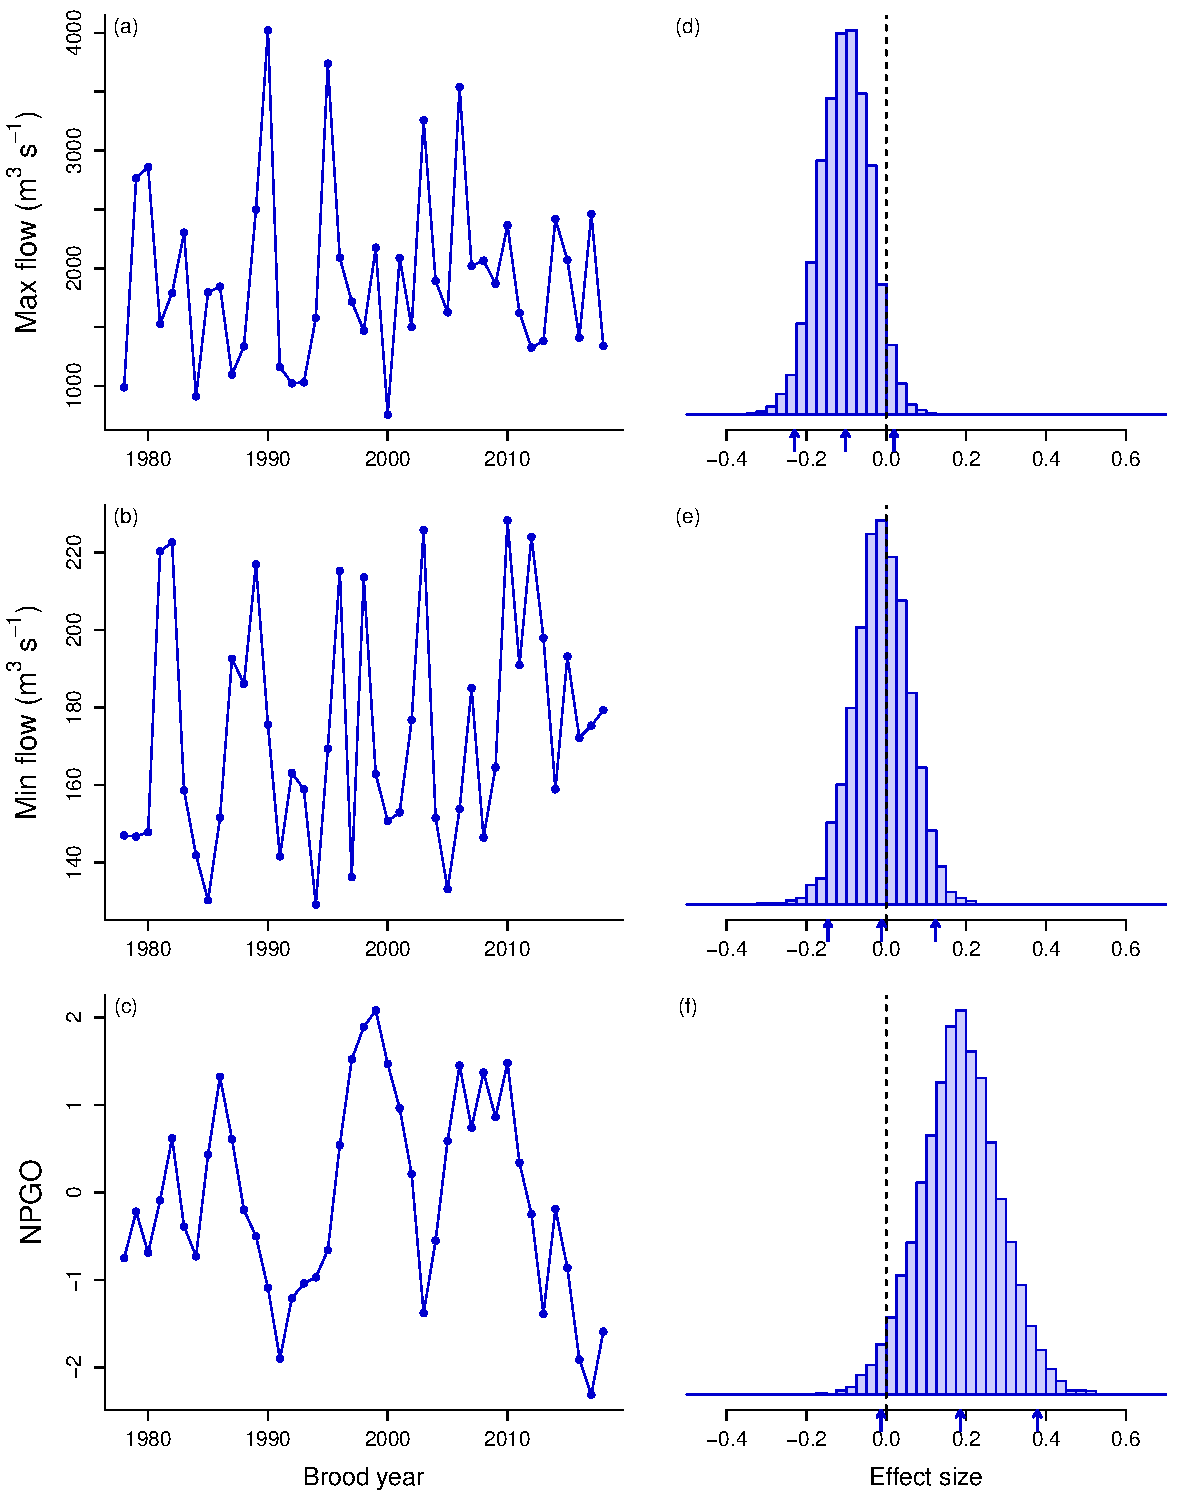
\includegraphics{App_3_Summarize_results_forecast_2020_2021_files/figure-latex/fig_4_cov_effects-1} \end{center}

Figure 3: Time series of the environmental covariates used in the model
(a-d), and their estimated effects on population productivity (e-g).
Small arrows under histograms denote 2.5\(^\text{th}\),
50\(^\text{th}\), and 97.5\(^\text{th}\) percentiles of the posterior
distribution.

Here is a summary of the covariate effect sizes

\begin{Shaded}
\begin{Highlighting}[]
\NormalTok{gamma_CI <-}\StringTok{ }\KeywordTok{apply}\NormalTok{(c_est, }\DecValTok{2}\NormalTok{, quantile, }\KeywordTok{c}\NormalTok{(}\FloatTok{2.5}\NormalTok{, }\DecValTok{5}\NormalTok{, }\DecValTok{50}\NormalTok{, }\DecValTok{95}\NormalTok{, }\FloatTok{97.5}\NormalTok{)}\OperatorTok{/}\DecValTok{100}\NormalTok{)}
\KeywordTok{t}\NormalTok{(}\KeywordTok{round}\NormalTok{(gamma_CI, }\DecValTok{2}\NormalTok{))}
\end{Highlighting}
\end{Shaded}

\begin{verbatim}
##           2.5%    5%   50%  95% 97.5%
## gamma[1] -0.23 -0.21 -0.10 0.00  0.02
## gamma[2] -0.15 -0.13 -0.01 0.10  0.12
## gamma[3] -0.01  0.02  0.19 0.35  0.38
\end{verbatim}

\hypertarget{process-errors}{%
\subsection{Process errors}\label{process-errors}}

Here is the time series of the residuals from the process model. They
represent the population's productivity after accounting for the effects
of density dependence and environmental covariates.

\begin{Shaded}
\begin{Highlighting}[]
\CommentTok{## time sequence}
\NormalTok{t_idx_a <-}\StringTok{ }\KeywordTok{seq}\NormalTok{(yr_frst, }\DataTypeTok{length.out =}\NormalTok{ n_yrs}\OperatorTok{-}\NormalTok{age_min}\OperatorTok{+}\NormalTok{n_fore)}
\CommentTok{## plot data}
\NormalTok{p_dat <-}\StringTok{ }\NormalTok{mod_res_MA1_AR1[,}\KeywordTok{grep}\NormalTok{(}\StringTok{"res_ln_Rec"}\NormalTok{, }\KeywordTok{colnames}\NormalTok{(mod_res_MA1_AR1))]}\OperatorTok{*}\NormalTok{model_weights[}\DecValTok{1}\NormalTok{] }\OperatorTok{+}\StringTok{ }\NormalTok{mod_res_AR1[,}\KeywordTok{grep}\NormalTok{(}\StringTok{"res_ln_Rec"}\NormalTok{, }\KeywordTok{colnames}\NormalTok{(mod_res_AR1))]}\OperatorTok{*}\NormalTok{model_weights[}\DecValTok{2}\NormalTok{] }

\NormalTok{p_dat <-}\StringTok{ }\KeywordTok{apply}\NormalTok{(p_dat, }\DecValTok{2}\NormalTok{, quantile, CI_vec)}
\NormalTok{yp_min <-}\StringTok{ }\KeywordTok{min}\NormalTok{(p_dat)}
\NormalTok{yp_max <-}\StringTok{ }\KeywordTok{max}\NormalTok{(p_dat)}
\CommentTok{## plot}
\KeywordTok{par}\NormalTok{(}\DataTypeTok{mai =} \KeywordTok{c}\NormalTok{(}\FloatTok{0.8}\NormalTok{,}\FloatTok{0.8}\NormalTok{,}\FloatTok{0.1}\NormalTok{,}\FloatTok{0.1}\NormalTok{), }\DataTypeTok{omi =} \KeywordTok{c}\NormalTok{(}\DecValTok{0}\NormalTok{,}\FloatTok{0.2}\NormalTok{,}\FloatTok{0.1}\NormalTok{,}\FloatTok{0.2}\NormalTok{))}
\KeywordTok{plot}\NormalTok{(t_idx_a, p_dat[}\DecValTok{3}\NormalTok{,],}
     \DataTypeTok{type =} \StringTok{"n"}\NormalTok{,  }\DataTypeTok{bty =} \StringTok{"L"}\NormalTok{,}
     \DataTypeTok{ylim =} \KeywordTok{c}\NormalTok{(yp_min,yp_max),}
     \DataTypeTok{xlab =} \StringTok{"Brood year"}\NormalTok{, }\DataTypeTok{ylab =} \StringTok{"Process error"}\NormalTok{, }\DataTypeTok{main =} \StringTok{""}\NormalTok{,}
     \DataTypeTok{cex.lab =} \FloatTok{1.2}\NormalTok{)}
\KeywordTok{abline}\NormalTok{(}\DataTypeTok{h =} \DecValTok{0}\NormalTok{, }\DataTypeTok{lty =} \StringTok{"dashed"}\NormalTok{)}
\KeywordTok{polygon}\NormalTok{(}\KeywordTok{c}\NormalTok{(t_idx_a, }\KeywordTok{rev}\NormalTok{(t_idx_a)), }\KeywordTok{c}\NormalTok{(p_dat[}\DecValTok{3}\NormalTok{,], }\KeywordTok{rev}\NormalTok{(p_dat[}\DecValTok{1}\NormalTok{,])),}
        \DataTypeTok{col =}\NormalTok{ clr, }\DataTypeTok{border =} \OtherTok{NA}\NormalTok{)}
\KeywordTok{lines}\NormalTok{(t_idx_a, p_dat[}\DecValTok{2}\NormalTok{,], }\DataTypeTok{col =} \StringTok{"blue3"}\NormalTok{, }\DataTypeTok{lwd =} \DecValTok{2}\NormalTok{)}
\end{Highlighting}
\end{Shaded}

\begin{center}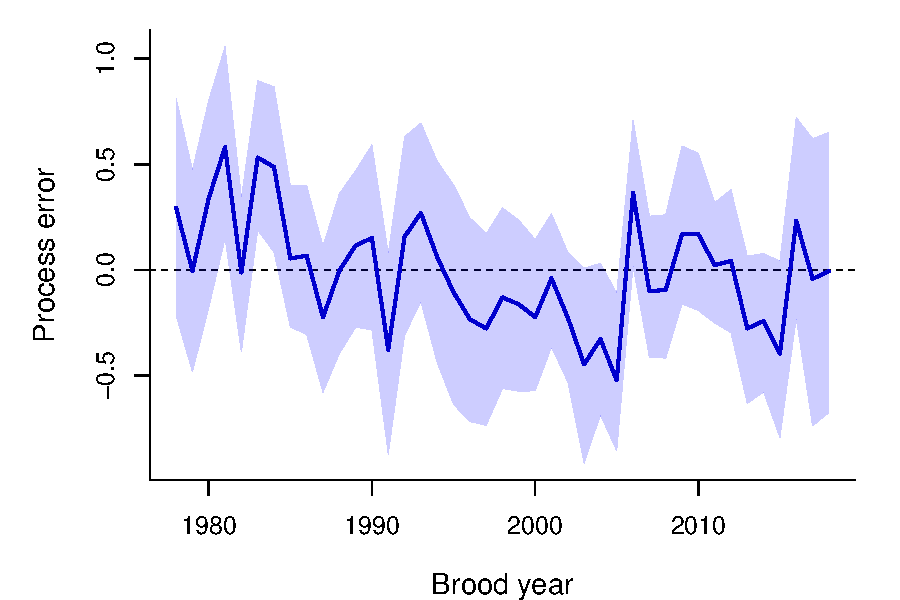
\includegraphics{App_3_Summarize_results_forecast_2020_2021_files/figure-latex/fig_5_proc_err-1} \end{center}

Figure 4: Time series of the estimated process errors, which represent
the population's productivity after accounting for the effects of
density dependence and environmental covariates. The solid line is the
median estimate and the shaded region indicates the 95\% credible
interval.

\hypertarget{management-reference-points}{%
\subsection{Management reference
points}\label{management-reference-points}}

Here are a number of management reference points.

\begin{Shaded}
\begin{Highlighting}[]
\CommentTok{## abbreviations for ref points}
\NormalTok{ref_names <-}\StringTok{ }\KeywordTok{c}\NormalTok{(}\StringTok{"MSY"}\NormalTok{, }\StringTok{"Smsy"}\NormalTok{, }\StringTok{"Umsy"}\NormalTok{, }\StringTok{"Umax"}\NormalTok{)}
\CommentTok{## proportions of MSY to consider}
\NormalTok{yld_prop <-}\StringTok{ }\KeywordTok{c}\NormalTok{(}\FloatTok{0.75}\NormalTok{, }\FloatTok{0.85}\NormalTok{, }\FloatTok{0.95}\NormalTok{)}
\CommentTok{## median values for a & b}
\NormalTok{aa <-}\StringTok{ }\NormalTok{mod_res_MA1_AR1[,}\KeywordTok{grep}\NormalTok{(}\StringTok{"E_BH_a"}\NormalTok{, }\KeywordTok{colnames}\NormalTok{(mod_res_MA1_AR1))]}\OperatorTok{*}\NormalTok{model_weights[}\DecValTok{1}\NormalTok{] }\OperatorTok{+}\StringTok{ }\NormalTok{mod_res_AR1[,}\KeywordTok{grep}\NormalTok{(}\StringTok{"E_BH_a"}\NormalTok{, }\KeywordTok{colnames}\NormalTok{(mod_res_AR1))]}\OperatorTok{*}\NormalTok{model_weights[}\DecValTok{2}\NormalTok{] }

\NormalTok{alpha <-}\StringTok{ }\KeywordTok{exp}\NormalTok{(aa)}
\NormalTok{mcmc <-}\StringTok{ }\KeywordTok{length}\NormalTok{(aa)}

\NormalTok{beta <-}\StringTok{ }\NormalTok{mod_res_MA1_AR1[,}\KeywordTok{grep}\NormalTok{(}\StringTok{"beta"}\NormalTok{, }\KeywordTok{colnames}\NormalTok{(mod_res_MA1_AR1))]}\OperatorTok{*}\NormalTok{model_weights[}\DecValTok{1}\NormalTok{] }\OperatorTok{+}\StringTok{ }\NormalTok{mod_res_AR1[,}\KeywordTok{grep}\NormalTok{(}\StringTok{"beta"}\NormalTok{, }\KeywordTok{colnames}\NormalTok{(mod_res_AR1))]}\OperatorTok{*}\NormalTok{model_weights[}\DecValTok{2}\NormalTok{] }

\CommentTok{## empty matrix for ref pts}
\NormalTok{ref_pts <-}\StringTok{ }\KeywordTok{matrix}\NormalTok{(}\OtherTok{NA}\NormalTok{, mcmc, }\KeywordTok{length}\NormalTok{(ref_names))}
\KeywordTok{colnames}\NormalTok{(ref_pts) <-}\StringTok{ }\NormalTok{ref_names}
\CommentTok{## spawner series for optimal yield profile}
\NormalTok{SS <-}\StringTok{ }\KeywordTok{seq}\NormalTok{(}\DecValTok{100}\NormalTok{, }\FloatTok{1e4}\NormalTok{, }\DecValTok{100}\NormalTok{)}
\CommentTok{## empty matrix for optimal yield profiles}
\NormalTok{OYP <-}\StringTok{ }\KeywordTok{matrix}\NormalTok{(}\DecValTok{0}\NormalTok{, }\KeywordTok{length}\NormalTok{(SS), }\KeywordTok{length}\NormalTok{(yld_prop))}
\ControlFlowTok{for}\NormalTok{(i }\ControlFlowTok{in} \DecValTok{1}\OperatorTok{:}\NormalTok{mcmc) \{}
    \CommentTok{## spawners at MSY}
\NormalTok{    ref_pts[i, }\StringTok{"Smsy"}\NormalTok{] <-}\StringTok{ }\NormalTok{(alpha[i] }\OperatorTok{/}\StringTok{ }\NormalTok{beta[i]) }\OperatorTok{*}\StringTok{ }\KeywordTok{sqrt}\NormalTok{(}\DecValTok{1} \OperatorTok{/}\StringTok{ }\NormalTok{alpha[i]) }\OperatorTok{-}\StringTok{ }\NormalTok{(}\DecValTok{1} \OperatorTok{/}\StringTok{ }\NormalTok{beta[i])}
    \CommentTok{## MSY}
\NormalTok{    ref_pts[i, }\StringTok{"MSY"}\NormalTok{] <-}\StringTok{ }\NormalTok{(ref_pts[i,}\StringTok{"Smsy"}\NormalTok{] }\OperatorTok{*}\StringTok{ }\NormalTok{alpha[i]) }\OperatorTok{/}
\StringTok{                            }\NormalTok{(}\DecValTok{1} \OperatorTok{+}\StringTok{ }\NormalTok{beta[i] }\OperatorTok{*}\StringTok{ }\NormalTok{ref_pts[i, }\StringTok{"Smsy"}\NormalTok{]) }\OperatorTok{-}\StringTok{ }\NormalTok{ref_pts[i, }\StringTok{"Smsy"}\NormalTok{]}
    \CommentTok{## harvest rate at MSY}
\NormalTok{    ref_pts[i, }\StringTok{"Umsy"}\NormalTok{] <-}\StringTok{ }\DecValTok{1} \OperatorTok{-}\StringTok{ }\KeywordTok{sqrt}\NormalTok{(}\DecValTok{1} \OperatorTok{/}\StringTok{ }\NormalTok{alpha[i])}
    \CommentTok{## max harvest rate}
\NormalTok{    ref_pts[i, }\StringTok{"Umax"}\NormalTok{] <-}\StringTok{ }\DecValTok{1} \OperatorTok{-}\StringTok{ }\DecValTok{1}\OperatorTok{/}\NormalTok{alpha[i]}
    \CommentTok{## yield over varying S}
\NormalTok{    yield <-}\StringTok{ }\NormalTok{((SS }\OperatorTok{*}\StringTok{ }\NormalTok{alpha[i]) }\OperatorTok{/}\StringTok{ }\NormalTok{(}\DecValTok{1} \OperatorTok{+}\StringTok{ }\NormalTok{beta[i] }\OperatorTok{*}\StringTok{ }\NormalTok{SS)) }\OperatorTok{-}\StringTok{ }\NormalTok{SS}
    \ControlFlowTok{for}\NormalTok{(j }\ControlFlowTok{in} \DecValTok{1}\OperatorTok{:}\KeywordTok{length}\NormalTok{(yld_prop)) \{}
\NormalTok{        OYP[,j] <-}\StringTok{ }\NormalTok{OYP[,j] }\OperatorTok{+}\StringTok{ }\DecValTok{1}\OperatorTok{*}\NormalTok{(yield }\OperatorTok{>}\StringTok{ }\NormalTok{yld_prop[j] }\OperatorTok{*}\StringTok{ }\NormalTok{ref_pts[i, }\StringTok{"MSY"}\NormalTok{])}
\NormalTok{    \}}
\NormalTok{\}}
\NormalTok{OYP <-}\StringTok{ }\NormalTok{OYP}\OperatorTok{/}\NormalTok{mcmc}

\CommentTok{## Prob of overfishing}
\NormalTok{hh <-}\StringTok{ }\KeywordTok{seq}\NormalTok{(}\DecValTok{100}\NormalTok{)}
\NormalTok{Pr_over <-}\StringTok{ }\KeywordTok{cbind}\NormalTok{(hh,hh,hh)}
\KeywordTok{colnames}\NormalTok{(Pr_over) <-}\StringTok{ }\KeywordTok{c}\NormalTok{(}\StringTok{"Umsy75"}\NormalTok{,}\StringTok{"Umsy"}\NormalTok{,}\StringTok{"Umax"}\NormalTok{)}
\ControlFlowTok{for}\NormalTok{(i }\ControlFlowTok{in}\NormalTok{ hh) \{}
\NormalTok{  Pr_over[i,}\StringTok{"Umsy75"}\NormalTok{] <-}\StringTok{ }\KeywordTok{sum}\NormalTok{(ref_pts[,}\StringTok{"Umsy"}\NormalTok{] }\OperatorTok{*}\StringTok{ }\FloatTok{0.75} \OperatorTok{<}\StringTok{ }\NormalTok{i}\OperatorTok{/}\DecValTok{100}\NormalTok{)}\OperatorTok{/}\NormalTok{mcmc}
\NormalTok{  Pr_over[i,}\StringTok{"Umsy"}\NormalTok{] <-}\StringTok{ }\KeywordTok{sum}\NormalTok{(ref_pts[,}\StringTok{"Umsy"}\NormalTok{] }\OperatorTok{<}\StringTok{ }\NormalTok{i}\OperatorTok{/}\DecValTok{100}\NormalTok{)}\OperatorTok{/}\NormalTok{mcmc}
\NormalTok{  Pr_over[i,}\StringTok{"Umax"}\NormalTok{] <-}\StringTok{ }\KeywordTok{sum}\NormalTok{(ref_pts[,}\StringTok{"Umax"}\NormalTok{] }\OperatorTok{<}\StringTok{ }\NormalTok{i}\OperatorTok{/}\DecValTok{100}\NormalTok{)}\OperatorTok{/}\NormalTok{mcmc}
\NormalTok{\}}

\CommentTok{## posterior exploitation rate & spawner abundance}

\NormalTok{aer <-}\StringTok{ }\NormalTok{Sp_ts <-}\StringTok{ }\NormalTok{mod_res_MA1_AR1[,}\KeywordTok{grep}\NormalTok{(}\StringTok{"Sp"}\NormalTok{, }\KeywordTok{colnames}\NormalTok{(mod_res_MA1_AR1))]}\OperatorTok{*}\NormalTok{model_weights[}\DecValTok{1}\NormalTok{] }\OperatorTok{+}\StringTok{ }\NormalTok{mod_res_AR1[,}\KeywordTok{grep}\NormalTok{(}\StringTok{"Sp"}\NormalTok{, }\KeywordTok{colnames}\NormalTok{(mod_res_AR1))]}\OperatorTok{*}\NormalTok{model_weights[}\DecValTok{2}\NormalTok{] }
\NormalTok{aer <-}\StringTok{ }\NormalTok{aer[,}\DecValTok{1}\OperatorTok{:}\NormalTok{n_yrs]}
\ControlFlowTok{for}\NormalTok{(i }\ControlFlowTok{in} \DecValTok{1}\OperatorTok{:}\NormalTok{n_yrs) \{}
\NormalTok{    aer[,i] <-}\StringTok{ }\NormalTok{dat_harv[i] }\OperatorTok{/}\StringTok{ }\NormalTok{(dat_harv[i] }\OperatorTok{+}\StringTok{ }\NormalTok{Sp_ts[,i]) }
\NormalTok{\}}
\end{Highlighting}
\end{Shaded}

\begin{Shaded}
\begin{Highlighting}[]
\KeywordTok{layout}\NormalTok{(}\KeywordTok{matrix}\NormalTok{(}\KeywordTok{c}\NormalTok{(}\DecValTok{2}\NormalTok{, }\DecValTok{1}\NormalTok{, }\DecValTok{4}\NormalTok{, }\DecValTok{3}\NormalTok{), }\DecValTok{2}\NormalTok{, }\DecValTok{2}\NormalTok{), }\DataTypeTok{heights =} \KeywordTok{c}\NormalTok{(}\DecValTok{1}\NormalTok{, }\DecValTok{5}\NormalTok{))}
\NormalTok{yoffSet <-}\StringTok{ }\FloatTok{0.10}
\NormalTok{yoffSet <-}\StringTok{ }\FloatTok{0.05}

\CommentTok{## (a) Optimal yield profile}
\KeywordTok{par}\NormalTok{(}\DataTypeTok{mai=}\KeywordTok{c}\NormalTok{(}\FloatTok{0.9}\NormalTok{, }\FloatTok{0.9}\NormalTok{, }\DecValTok{0}\NormalTok{, }\DecValTok{0}\NormalTok{), }\DataTypeTok{omi=}\KeywordTok{c}\NormalTok{(}\DecValTok{0}\NormalTok{, }\DecValTok{0}\NormalTok{, }\FloatTok{0.1}\NormalTok{, }\FloatTok{0.1}\NormalTok{))}
\NormalTok{x_lp <-}\StringTok{ }\NormalTok{yld_prop}
\ControlFlowTok{for}\NormalTok{(i }\ControlFlowTok{in} \DecValTok{1}\OperatorTok{:}\KeywordTok{length}\NormalTok{(x_lp)) \{}
\NormalTok{    x_lp[i] <-}\StringTok{ }\NormalTok{SS[}\KeywordTok{max}\NormalTok{(}\KeywordTok{which}\NormalTok{(OYP[,i] }\OperatorTok{==}\StringTok{ }\KeywordTok{max}\NormalTok{(OYP[,i])}
                            \OperatorTok{|}\StringTok{ }\KeywordTok{abs}\NormalTok{(OYP[,i] }\OperatorTok{-}\StringTok{ }\NormalTok{(yld_prop[i]}\OperatorTok{-}\FloatTok{0.3}\NormalTok{)) }\OperatorTok{<=}\StringTok{ }\FloatTok{0.05}\NormalTok{))]}
\NormalTok{\}}
\KeywordTok{matplot}\NormalTok{(SS, OYP, }\DataTypeTok{type=}\StringTok{"l"}\NormalTok{, }\DataTypeTok{lty=}\StringTok{"solid"}\NormalTok{,  }\DataTypeTok{ylim=}\KeywordTok{c}\NormalTok{(}\DecValTok{0}\NormalTok{,}\DecValTok{1}\NormalTok{),}
        \DataTypeTok{col=}\KeywordTok{c}\NormalTok{(}\StringTok{"slateblue"}\NormalTok{,}\StringTok{"blue"}\NormalTok{,}\StringTok{"darkblue"}\NormalTok{), }\DataTypeTok{lwd=}\DecValTok{2}\NormalTok{,}
        \DataTypeTok{xlab =} \StringTok{"Spawners"}\NormalTok{, }\DataTypeTok{ylab =} \StringTok{"Probability of X% of MSY"}\NormalTok{, }\DataTypeTok{main =} \StringTok{""}\NormalTok{,}
        \DataTypeTok{las=}\DecValTok{1}\NormalTok{, }\DataTypeTok{cex.lab=}\FloatTok{1.2}\NormalTok{)}
\KeywordTok{points}\NormalTok{(}\DataTypeTok{x =}\NormalTok{ x_lp, }\DataTypeTok{y =}\NormalTok{ yld_prop}\FloatTok{-0.3}\NormalTok{,}
       \DataTypeTok{pch =} \DecValTok{21}\NormalTok{, }\DataTypeTok{cex =} \FloatTok{3.5}\NormalTok{,}
       \DataTypeTok{col =} \StringTok{"white"}\NormalTok{, }\DataTypeTok{bg =} \StringTok{"white"}\NormalTok{)}
\KeywordTok{text}\NormalTok{(}\DataTypeTok{x =}\NormalTok{ x_lp, }\DataTypeTok{y =}\NormalTok{ yld_prop}\FloatTok{-0.3}\NormalTok{, }\KeywordTok{paste0}\NormalTok{(yld_prop}\OperatorTok{*}\DecValTok{100}\NormalTok{, }\StringTok{"%"}\NormalTok{),}
     \DataTypeTok{col=}\KeywordTok{c}\NormalTok{(}\StringTok{"slateblue"}\NormalTok{,}\StringTok{"blue"}\NormalTok{,}\StringTok{"darkblue"}\NormalTok{), }\DataTypeTok{cex=}\FloatTok{0.7}\NormalTok{)}
\KeywordTok{text}\NormalTok{(}\DataTypeTok{x =} \KeywordTok{par}\NormalTok{()}\OperatorTok{$}\NormalTok{usr[}\DecValTok{1}\NormalTok{] }\OperatorTok{+}\StringTok{ }\NormalTok{xoffSet }\OperatorTok{*}\StringTok{ }\KeywordTok{diff}\NormalTok{(}\KeywordTok{par}\NormalTok{()}\OperatorTok{$}\NormalTok{usr[}\DecValTok{1}\OperatorTok{:}\DecValTok{2}\NormalTok{]),}
     \DataTypeTok{y =} \KeywordTok{par}\NormalTok{()}\OperatorTok{$}\NormalTok{usr[}\DecValTok{4}\NormalTok{] }\OperatorTok{-}\StringTok{ }\NormalTok{yoffSet }\OperatorTok{*}\StringTok{ }\KeywordTok{diff}\NormalTok{(}\KeywordTok{par}\NormalTok{()}\OperatorTok{$}\NormalTok{usr[}\DecValTok{3}\OperatorTok{:}\DecValTok{4}\NormalTok{]),}
     \StringTok{"(a)"}\NormalTok{)}
\CommentTok{## marginal histogram of posterior spawner abundances}
\KeywordTok{par}\NormalTok{(}\DataTypeTok{mai=}\KeywordTok{c}\NormalTok{(}\DecValTok{0}\NormalTok{, }\FloatTok{0.9}\NormalTok{, }\FloatTok{0.05}\NormalTok{, }\DecValTok{0}\NormalTok{))}
\KeywordTok{hist}\NormalTok{(Sp_ts[Sp_ts}\OperatorTok{<}\FloatTok{1e4}\NormalTok{], }\DataTypeTok{breaks =} \DecValTok{40}\NormalTok{,}
     \DataTypeTok{col =}\NormalTok{ clr, }\DataTypeTok{border =} \StringTok{"blue3"}\NormalTok{, }
     \DataTypeTok{yaxs =} \StringTok{"i"}\NormalTok{, }\DataTypeTok{xaxt =} \StringTok{"n"}\NormalTok{, }\DataTypeTok{yaxt =} \StringTok{"n"}\NormalTok{,}
     \DataTypeTok{main =} \StringTok{""}\NormalTok{, }\DataTypeTok{ylab =} \StringTok{""}\NormalTok{)}

\CommentTok{## (b) Probability of overfishing}
\KeywordTok{par}\NormalTok{(}\DataTypeTok{mai=}\KeywordTok{c}\NormalTok{(}\FloatTok{0.9}\NormalTok{, }\FloatTok{0.9}\NormalTok{, }\DecValTok{0}\NormalTok{, }\DecValTok{0}\NormalTok{))}
\KeywordTok{matplot}\NormalTok{(Pr_over, }\DataTypeTok{type =} \StringTok{"l"}\NormalTok{, }\DataTypeTok{lwd =} \DecValTok{2}\NormalTok{, }\DataTypeTok{lty =} \StringTok{"solid"}\NormalTok{,}
        \DataTypeTok{col =} \KeywordTok{c}\NormalTok{(}\StringTok{"slateblue"}\NormalTok{,}\StringTok{"blue"}\NormalTok{,}\StringTok{"darkblue"}\NormalTok{), }
        \DataTypeTok{ylab=}\StringTok{"Probability of overfishing"}\NormalTok{, }
        \DataTypeTok{xlab=}\StringTok{"Harvest rate"}\NormalTok{, }\DataTypeTok{xaxt=}\StringTok{"n"}\NormalTok{,}
        \DataTypeTok{las =} \DecValTok{1}\NormalTok{, }\DataTypeTok{cex.lab =} \FloatTok{1.2}\NormalTok{)}
\KeywordTok{axis}\NormalTok{(}\DecValTok{1}\NormalTok{, }\KeywordTok{seq}\NormalTok{(}\DecValTok{0}\NormalTok{,}\DecValTok{100}\NormalTok{,}\DecValTok{20}\NormalTok{), }\KeywordTok{seq}\NormalTok{(}\DecValTok{0}\NormalTok{,}\DecValTok{100}\NormalTok{,}\DecValTok{20}\NormalTok{)}\OperatorTok{/}\DecValTok{100}\NormalTok{)}
\NormalTok{x_lp <-}\StringTok{ }\KeywordTok{c}\NormalTok{(}\DecValTok{0}\NormalTok{, }\DecValTok{0}\NormalTok{, }\DecValTok{0}\NormalTok{)}
\ControlFlowTok{for}\NormalTok{(i }\ControlFlowTok{in} \DecValTok{1}\OperatorTok{:}\KeywordTok{length}\NormalTok{(x_lp)) \{}
\NormalTok{  x_lp[i] <-}\StringTok{ }\KeywordTok{max}\NormalTok{(}\KeywordTok{which}\NormalTok{(}\KeywordTok{abs}\NormalTok{(Pr_over[,i] }\OperatorTok{-}\StringTok{ }\FloatTok{0.5}\NormalTok{) }\OperatorTok{<=}\StringTok{ }\FloatTok{0.05}\NormalTok{))}
\NormalTok{\}}
\KeywordTok{points}\NormalTok{(}\DataTypeTok{x =}\NormalTok{ x_lp, }\DataTypeTok{y =} \KeywordTok{rep}\NormalTok{(}\FloatTok{0.5}\NormalTok{, }\DecValTok{3}\NormalTok{), }\DataTypeTok{pch =} \DecValTok{21}\NormalTok{, }\DataTypeTok{cex =} \DecValTok{4}\NormalTok{,}
       \DataTypeTok{col =} \StringTok{"white"}\NormalTok{, }\DataTypeTok{bg =} \StringTok{"white"}\NormalTok{)}
\KeywordTok{text}\NormalTok{(}\DataTypeTok{x =}\NormalTok{ x_lp, }\DataTypeTok{y =} \FloatTok{0.5}\NormalTok{, }\KeywordTok{expression}\NormalTok{(U[M75], U[MSY], U[Max]),}
     \DataTypeTok{col =} \KeywordTok{c}\NormalTok{(}\StringTok{"slateblue"}\NormalTok{, }\StringTok{"blue"}\NormalTok{, }\StringTok{"darkblue"}\NormalTok{), }\DataTypeTok{cex =} \FloatTok{0.8}\NormalTok{)}
\KeywordTok{text}\NormalTok{(}\DataTypeTok{x =} \KeywordTok{par}\NormalTok{()}\OperatorTok{$}\NormalTok{usr[}\DecValTok{1}\NormalTok{] }\OperatorTok{+}\StringTok{ }\NormalTok{xoffSet }\OperatorTok{*}\StringTok{ }\KeywordTok{diff}\NormalTok{(}\KeywordTok{par}\NormalTok{()}\OperatorTok{$}\NormalTok{usr[}\DecValTok{1}\OperatorTok{:}\DecValTok{2}\NormalTok{]),}
     \DataTypeTok{y =} \KeywordTok{par}\NormalTok{()}\OperatorTok{$}\NormalTok{usr[}\DecValTok{4}\NormalTok{] }\OperatorTok{-}\StringTok{ }\NormalTok{yoffSet }\OperatorTok{*}\StringTok{ }\KeywordTok{diff}\NormalTok{(}\KeywordTok{par}\NormalTok{()}\OperatorTok{$}\NormalTok{usr[}\DecValTok{3}\OperatorTok{:}\DecValTok{4}\NormalTok{]),}
     \StringTok{"(b)"}\NormalTok{)}
\CommentTok{## marginal histogram of posterior harvest rates}
\KeywordTok{par}\NormalTok{(}\DataTypeTok{mai =} \KeywordTok{c}\NormalTok{(}\DecValTok{0}\NormalTok{ ,}\FloatTok{0.9}\NormalTok{, }\FloatTok{0.05}\NormalTok{, }\DecValTok{0}\NormalTok{))}
\KeywordTok{hist}\NormalTok{(aer, }\DataTypeTok{breaks =} \KeywordTok{seq}\NormalTok{(}\DecValTok{0}\NormalTok{, }\DecValTok{40}\NormalTok{)}\OperatorTok{/}\DecValTok{40}\NormalTok{,}
     \DataTypeTok{col =}\NormalTok{ clr, }\DataTypeTok{border =} \StringTok{"blue3"}\NormalTok{,}
     \DataTypeTok{yaxs =} \StringTok{"i"}\NormalTok{, }\DataTypeTok{xaxt =} \StringTok{"n"}\NormalTok{, }\DataTypeTok{yaxt =} \StringTok{"n"}\NormalTok{,}
     \DataTypeTok{main =} \StringTok{""}\NormalTok{, }\DataTypeTok{ylab =} \StringTok{""}\NormalTok{)}
\end{Highlighting}
\end{Shaded}

\begin{center}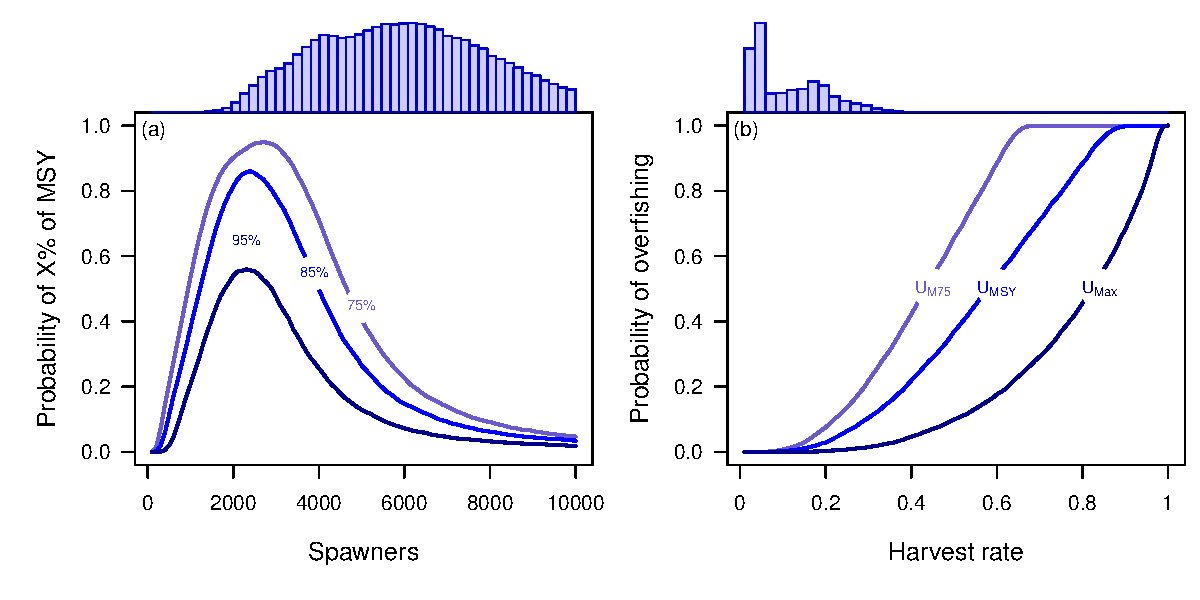
\includegraphics{App_3_Summarize_results_forecast_2020_2021_files/figure-latex/fig_6_ref_pts-1} \end{center}

Figure 5: Plots of (a) the probability that a given number of spawners
produces average yields achieving 95\%, 85\%, or 75\% of the estimated
maximum sustainable yield (MSY); and (b) the cumulative probability of
overfishing the population, based on harvest rates equal to those at
75\% of MSY, at MSY, and at the maximum per recruit. The histograms
above (a) and (b) are distributions of the posterior estimates for the
number of spawners and harvest rates, respectively; the histogram in (a)
has been truncated at \(10^4\).

\end{document}
